% Chapter Template

\chapter{Experimentally-generated ground truth for detecting cell types in an image-based immunotherapy screen} % Main chapter title

\label{Chapter4} % Change X to a consecutive number; for referencing this chapter elsewhere, use \ref{ChapterX}
\chaptermark{Experimentally-generated ground truth}

%\lhead{Chapter 2. \emph{Supervised Sequence Learning}} % Change X to a consecutive number; this is for the header on each page - perhaps a shortened title

\textbf{Summary}: \emph{Chimeric antigen receptor (CAR) is an immunotherapy whereby T lymphocytes are engineered to selectively attack cancer cells. Image-based screens of CAR-T cells, combining phase contrast and fluorescence microscopy, suffer from the gradual quenching of the fluorescent signal, making the reliable tracking of cell populations across time-lapse movies difficult. We propose to leverage the available fluorescent markers as an experimentally-generated ground truth. With some simple image processing, we are able to segment and assign cell type classes automatically. This ground truth is sufficient to train an object detection system from the phase contrast signal alone, potentially eliminating the need for the cumbersome fluorescent markers. This approach will underpin the development of cheap and robust microscope-based protocols to quantify CAR-T activity against tumor cell in vitro.}

\textbf{R\'esum\'e}: \emph{Cette chapitre...}

\section{Overview}

Chimeric antigen receptor T-cell (CAR-T) therapy is an immunotherapy whereby T lymphocytes (a subtype of white blood cells) are engineered to selectively attack cancer cells. Generally speaking, CARs are engineered or \emph{recombinant} receptors designed to target a specific protein, in practice a tumour antigen. When a CAR allows the CAR-T cell to latch onto an abnormal antigen, and deliver cytotoxic chemicals to induce \emph{lysis}  (membrane breakdown) of the target cell (\cite{benmebarek2019killing}). CAR technology has 30 years of development encompassing several design generations (\cite{maude2015cd19}).  As a therapy, T cells are extracted from a patient or healthy donor, modified (such as with viral transduction) to express the CAR in culture, and infused back into the patient. The \emph{in vivo} CAR-T cells then target tumours as a ``living drug'' treatment. The main engineering challenge is ensuring safety and efficacy, in particular the target specificity of the T cells (\cite{sadelainbasic}). CD19\footnote{Not to be confused with COVID-19.}, a B-cell surface protein is expressed by almost all B-cell cancers, such as acute lymphoblastic leukemia, one of the most common and fatal forms (primarily from relapse) of pediatric cancer worldwide (\cite{hunger2015acute}). In the latter disease, CD19 CAR-T has achieved up to $90\%$ complete remission rates in clinical studies such as \cite{maude2014chimeric}. Ideally, the antigen will be cancer-cell-specific, however CD19 CAR-T leads to B-cell \emph{aplasia}, that is, the depletion of B cells both cancerous and normal. Nevertheless, such side effects have been shown to be manageable (\cite{bonifant2016toxicity}). The pursuit of new forms of CAR is the subject of rapid and enthusiastic research (\cite{wang2017current}).

In a microscope setting where both transmitted light and fluorescence microscopy can be taken for the same cells simultaneously, interesting opportunities arise. Recently, successful attempts have been made (\cite{christiansen2018silico}, \cite{ounkomol2018label}) to predict fluorescent signals from transmitted light images, demonstrating that for certain biological experiments, the relevant information is wholly contained in the phase contrast signal. This is an attractive prospect because fluorescence microscopy, despite its power, has various drawbacks, with several experimental complications (such as fading dyes), in particular when imaging assays are performed over several days. In addition, the fluorescent marking of cells is expensive, time-consuming, and potentially invasive to the experiment. In this Chapter, we aim to leverage the fluorescent markers to quantify the cultured cells from the phase contrast alone. We compare two approaches to this quantification: the first, based on fluorescent labeling, is described in Section \label{sec:fluorescent_labeling}; the second, an object detection system, in Section \label{sec:object_detection_system}. In the part of the Chapter, we compare the two approaches.

\subsection{CAR-T dataset}

We obtained a set of time-lapse microscopy images from CAR-T experiments performed on an IncuCyte machine. In these experiments, the disease is modelled by Raji, an immortalised cell line of B lymphocytes from a $1963$ Burkitt's lymphoma patient. We study Raji cell populations in isolation, as well as cocultured with CAR-T cells. The setup is detailed in Table \ref{table:cart_plate}. The row A wells study isolated Raji cells; the row B wells study the coculture. Each well is imaged at $5\times$ magnification in four fields of view of size $1408\times1040$ pixels. Images were taken every two hours over a $220$ hour period ($110$ frames apiece) producing a time lapse movie. Each row of the microplate studied consists of two groups of two replicates, where each group has a different seeding quota. In our analysis, however, we consider the groups to be interchangeable and, where convenient, we pool data within each plate row. Each frame of each time lapse movie pairs a phase contrast image with green fluorescent protein (GFP) and mCherry fluorescent images, depicting the same scene. A sample is given in Figure \ref{fig:channels}. The mCherry fluorescence is present in all Raji cells while the GFP only appears in dead cells. The T cells, where present are only visible on the phase contrast channel. Thus, fluorescent markers combine for a quasi-annotation of the cells, which we may express with the (fuzzy) logic,

\begin{align}
\lnot \text{object} &\implies \text{background} \label{eq:fuzzy_logic} \\
\text{object} \land \text{GFP} &\implies \text{dead Raji} \nonumber \\
\text{object} \land \text{mCherry} \land \lnot \text{GFP} &\implies \text{Raji} \nonumber \\
\text{object} \land \lnot \text{mCherry} \land \lnot \text{GFP} &\implies \text{CAR-T} \nonumber
\end{align}

\begin{table}[h]
\centering
\begin{tabular}{|C{0.5cm}|C{2cm}|C{2cm}|C{2cm}|C{2cm}|} 
\hline
{} & 1 & 2 & 5 & 6 \\
\hline
\multicolumn{1}{|c|}{A} & \multicolumn{2}{p{4cm}|}{raji-target cells (1) 30K cells / well} & \multicolumn{2}{p{4cm}|}{raji-target cells (1) 30K cells / well} \\
\multicolumn{1}{|c|}{} & \multicolumn{2}{c|}{} & \multicolumn{2}{c|}{} \\
\hline
\multicolumn{1}{|c|}{B} & \multicolumn{2}{p{4cm}|}{CAR June 1:2 (1) 30K cells / well raji-target cells (1) 30K cells / well} & \multicolumn{2}{p{4cm}|}{CAR June 1:2 (1) 15K cells / well raji-target cells (1) 30K cells / well} \\
\multicolumn{1}{|c|}{} & \multicolumn{2}{c|}{} & \multicolumn{2}{c|}{} \\
\hline
\end{tabular}
\caption{Characteristics of CAR-T experiments studied. The . Row A studies RAJI cells in isolation; row B studies cocultured Raji and CAR-T cells.}
\label{table:cart_plate}
\end{table}

\begin{figure}[h]
\centering
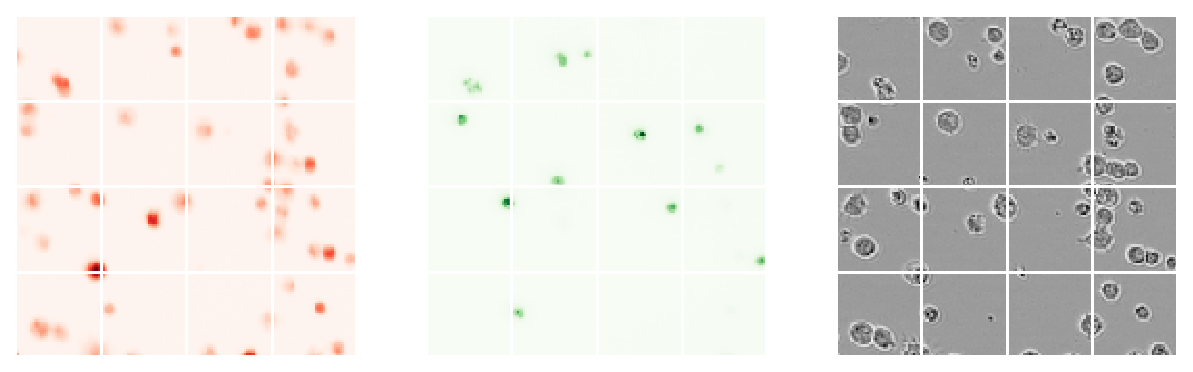
\includegraphics[width=\textwidth]{img/channels.pdf}
\label{fig:channels}
\caption{Aligned image channel crops ($200 \times200$px) marking living Raji cells in mCherry (left), dead cells in GFP (center), and phase contrast (right).}
\end{figure}

Note the high volume of data: the cells are seeded to a total of up to $60000$ per well, with four wells per experiment type, each with four fields and $110$ time lapse frames. Coupled with the fluorescence annotations, this is, in principle, a veritable treasure trove of data for deep learning. Annotation by experiment is a promising strategy: we can easily collect a large ground truth and, in addition, the ``experimental ground truth'' is much more objective than a manual one. A similar strategy has already been applied to image segmentation (\cite{sadanandan2017automated}). This seemingly overcomes the main bottleneck in leveraging deep learning models. However, this abundance of training data comes at a cost in resolution: most cells fit inside a $14 \times 14$ pixel window (contrast this with the much higher resolutions of our cells from Part \ref{partI}). This low resolution proves to be a constraint in the analyses to come, and an engineering challenge for our models.
\subsection{Experimental phenomena}
\label{subsec:phenomena}

Even at the best of times it is highly advisable to perform an exploratory analysis of a dataset. This principle served us well in Chapter \ref{Chapter2}, as we obtained important insights that we carried through to Chapter \ref{Chapter3}. With the temporal dimension now thrown in, the CAR-T dataset proves to be highly dynamic, and becomes increasingly chaotic in time, in particular as the Raji B-cells undergo mitosis. We presently detail some notable phenomena observable in our experimental data. These prove to be influential factors in our methodological designs.

\subsubsection{Apoptotic cells acquire GFP}

In Figure \ref{fig:dying_cell_frames} we trace the death of a Raji cell in full fluorescence. One may observe some subtle morphological changes such as a reduction in size, as well as a change of texture, which remain visible on the phase contrast channel. The fluorescence, however, shows a clear accumulation of GFP fluorophores. We measure the average intensity of each fluorescent channel in the cell region of interest and plot these over time in Figure \ref{fig:dying_cell_series}. The GFP signal rises for at least $10$ frames, corresponding to a $20$ hour period. The mCherry signal declines in time, seemingly in accordance with the quenching effect. We will see this latter phenomenon repeated elsewhere.

%
%\begin{figure}[h]
%\centering
%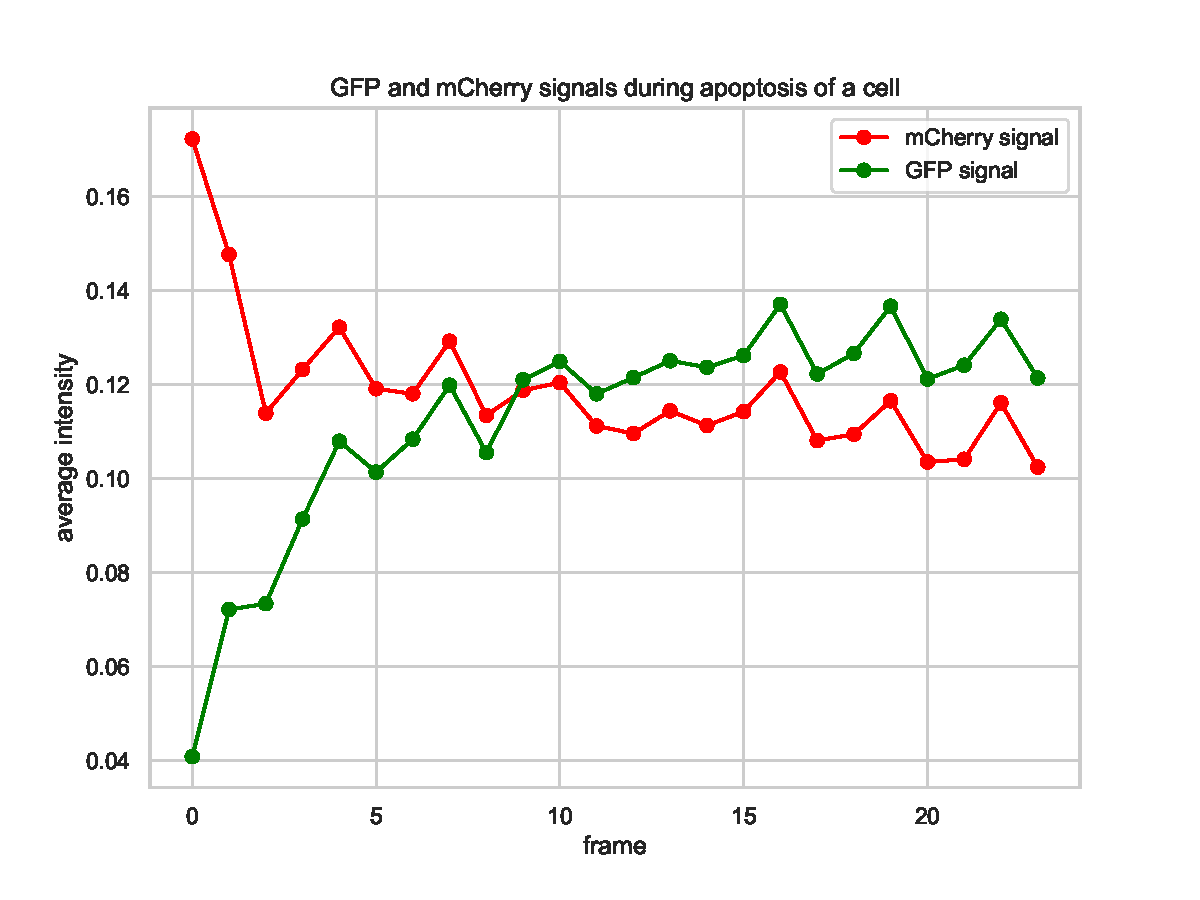
\includegraphics[width=0.85\textwidth]{img/dying_cell.pdf}
%\caption{Aligned image channel crops ($200 \times200$px) marking living Raji cells in mCherry (left), dead cells in GFP (center), and phase contrast (right).}
%\label{fig:dying_cell_graph}
%\end{figure}

\begin{figure*}[htb]
\centering
  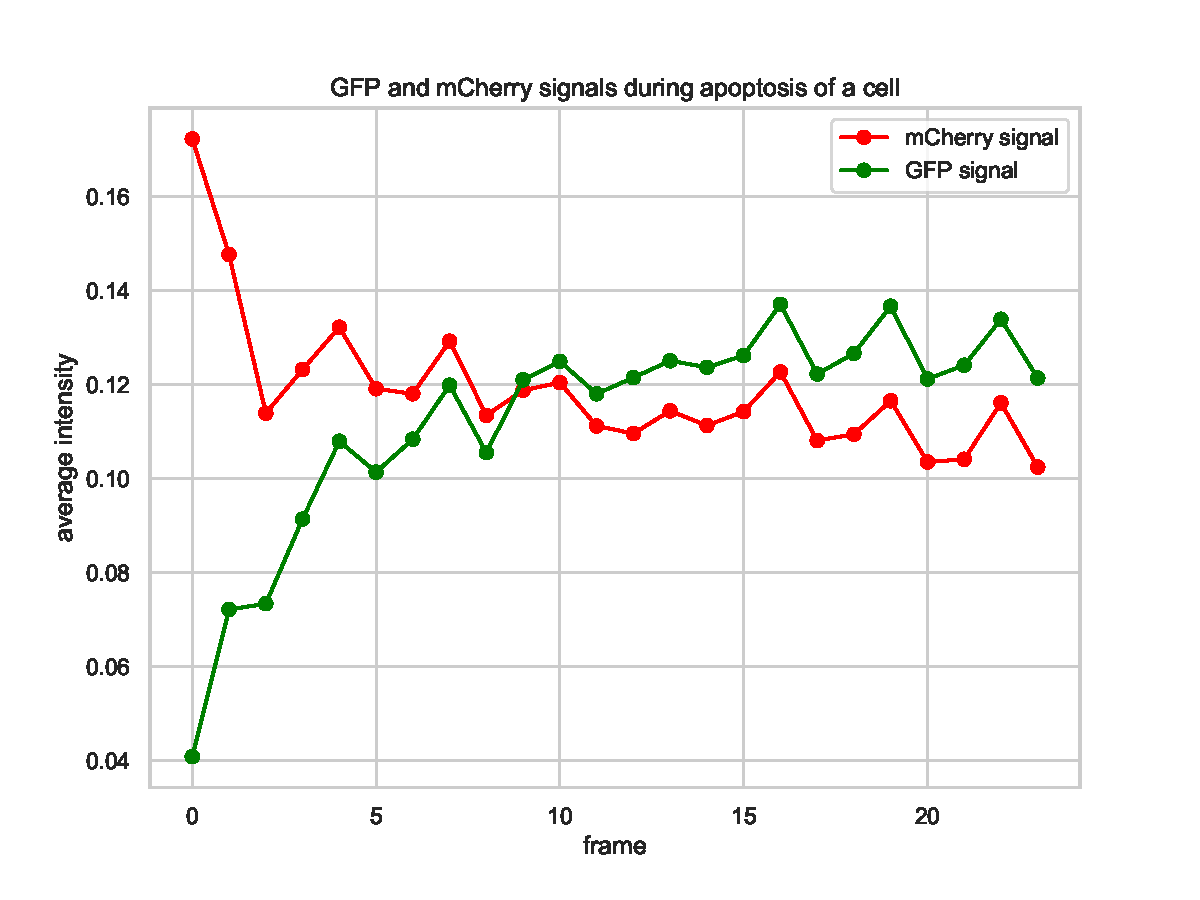
\includegraphics[width=\linewidth]{img/dying_cell.pdf}
  \caption{Tracking a mitotic event. The fluorescent turns green as a B cell undergoes morphological changes (a)-(f). This is reflected in a plot of intensity profiles (g).}
\label{fig:dying_cell_series}
\end{figure*}

%\begin{figure}[h!]%
%    \centering
%    \subfloat[\label{fig:dying_cell_frames_a}]{{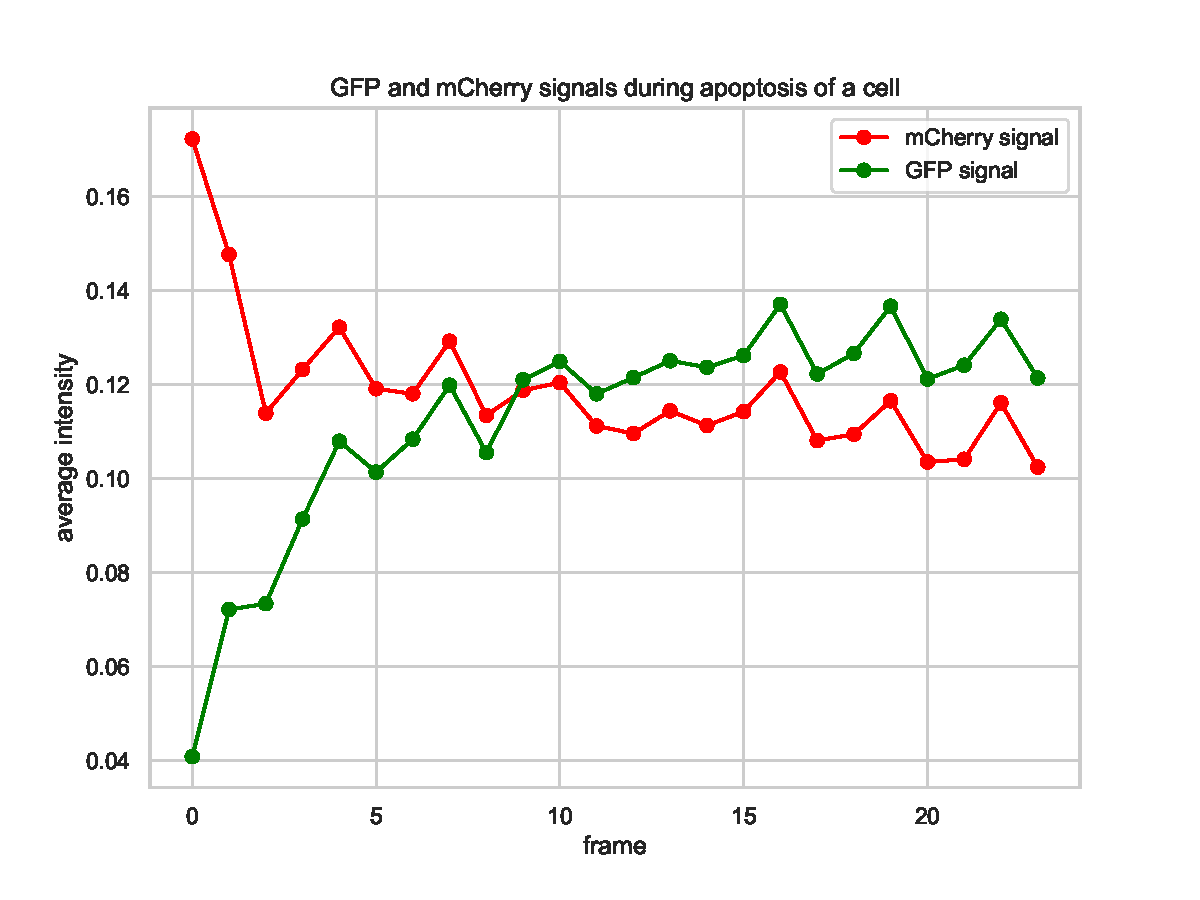
\includegraphics[width=0.9\textwidth]{img/dying_cell.pdf}}}
%	\qquad
%    \subfloat[\label{fig:dying_cell_frames_b}]{{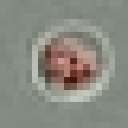
\includegraphics[width=.07\linewidth]{img/dying_cell_0000.png}}}%
%    \qquad
%    \subfloat[]{{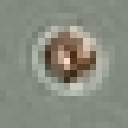
\includegraphics[width=.07\linewidth]{img/dying_cell_0001.png}}}%
%    \qquad
%    \subfloat[]{{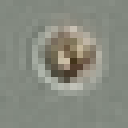
\includegraphics[width=.07\linewidth]{img/dying_cell_0002.png}}}%
%    \qquad
%    \subfloat[]{{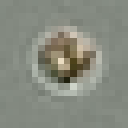
\includegraphics[width=.07\linewidth]{img/dying_cell_0003.png}}}%
%    \qquad
%    \subfloat[]{{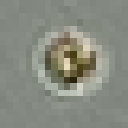
\includegraphics[width=.07\linewidth]{img/dying_cell_0004.png}}}%
%    \qquad
%    \subfloat[\label{fig:dying_cell_frames_g}]{{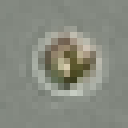
\includegraphics[width=.07\linewidth]{img/dying_cell_0005.png}}}%
%\caption{Tracking a mitotic event. The fluorescent turns green as a B cell undergoes morphological changes (a)-(f). This is reflected in a plot of intensity profiles (g).}
%\label{fig:dying_cell_frames}
%\end{figure}

\subsubsection{Raji mitosis creates cell clumps}

The phenomenon of mitosis or cell division greatly complicates the task of counting cells, and influences our methods in the current chapter as well as the next. It is well known that Raji cells group to form clusters or ``clumps'' (\cite{epstein1966morphological}). Figure \ref{fig:mitosis_frames} shows a sequence of cropped frames centered on a significant mitosis event. From a handful of dispersed cells in the initial frame $(t = 50)$, cell division occurs in time $(t = 70)$, $(t = 80)$, $(t = 90)$, creating clusters of closely touching, or even overlapping, cells. Whatever methodological approach we take, this complexifies the detection and segmentation individual cells as we can no longer utilise the image background to these ends. Whereas at first the cell contours are well-defined, the more the cells multiply, the less clear their separation, as cells begin to overlap.

\begin{figure}[h]%
    \centering
    \subfloat[$t=50$]{{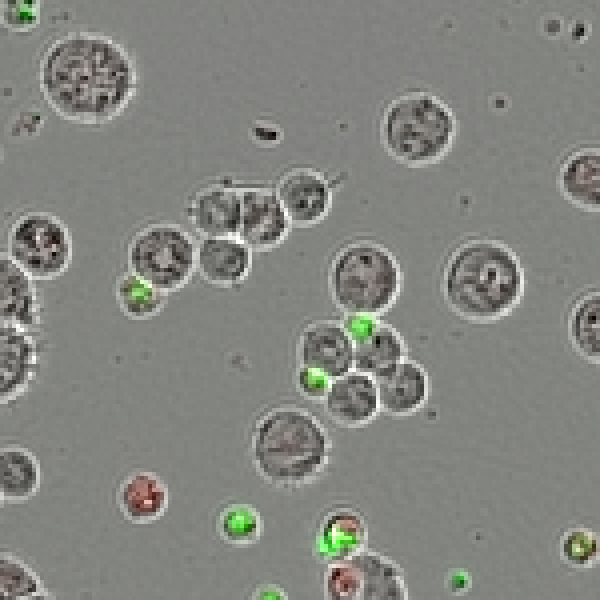
\includegraphics[width=.2\linewidth]{img/mitosis_25.png}}}%
    \qquad
    \subfloat[$t=70$]{{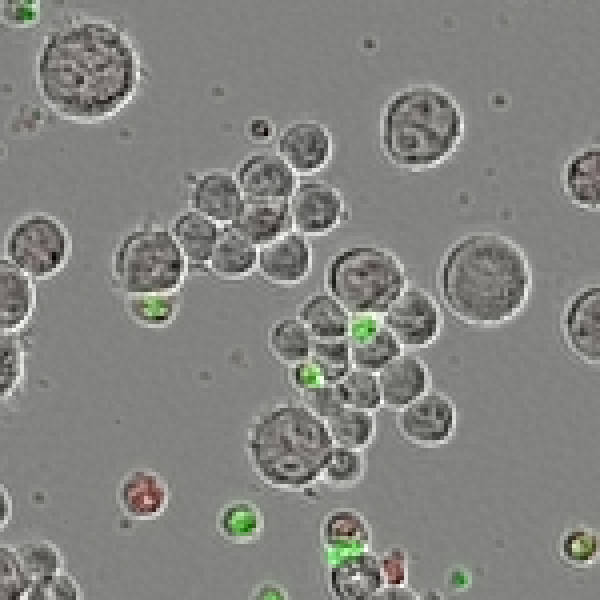
\includegraphics[width=.2\linewidth]{img/mitosis_35.png}}}%
    \qquad
    \subfloat[$t=80$]{{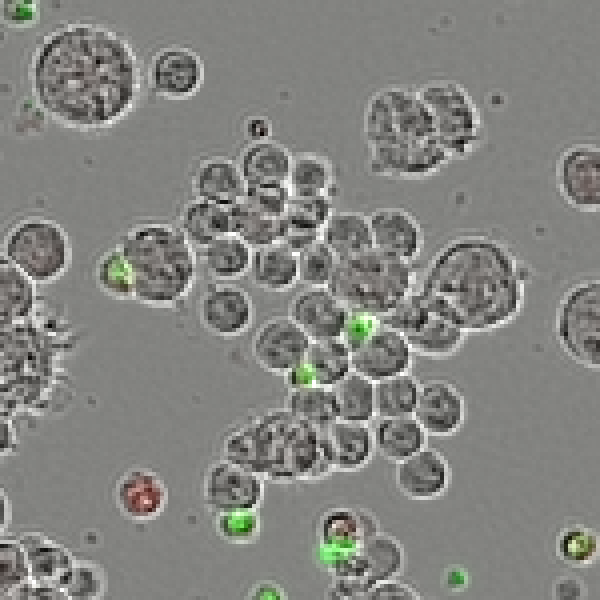
\includegraphics[width=.2\linewidth]{img/mitosis_40.png}}}%
	\qquad
    \subfloat[$t=90$]{{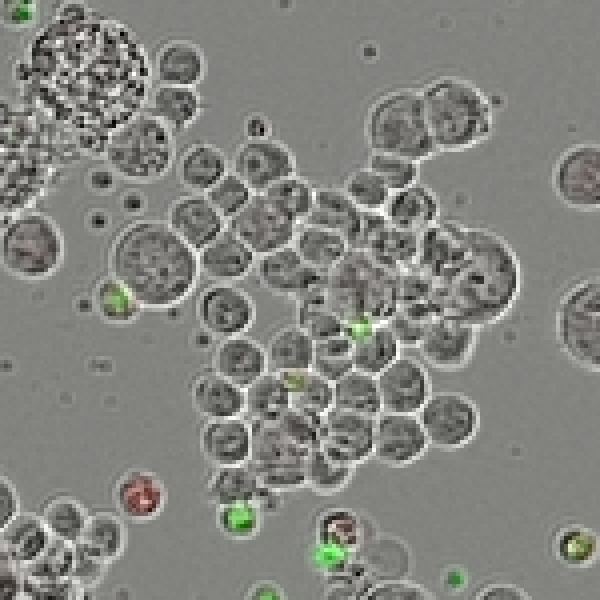
\includegraphics[width=.2\linewidth]{img/mitosis_45.png}}}%
\caption{Chronicling a mitotic event. Cells accumulate in clusters due to mitosis.}
\label{fig:mitosis_frames}
\end{figure}

\subsubsection{CAR-T cells create clusters of lysed target cells}

%\begin{figure}[h]%
%    \centering
%    \subfloat[]{{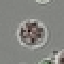
\includegraphics[width=.1\linewidth]{img/t_cell_21.png}}}%
%    \qquad
%    \subfloat[]{{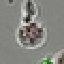
\includegraphics[width=.1\linewidth]{img/t_cell_22.png}}}%
%    \qquad
%    \subfloat[]{{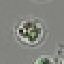
\includegraphics[width=.1\linewidth]{img/t_cell_46.png}}}%
%\caption{The processing of a test image: phase contrast input image (a); raw model bounding box predictions (b); non-maximum suppression post-processing (c); finally, for comparison, the corresponding full fluorescence image (d).}
%\label{fig:t_cell_frames}
%\end{figure}

With the inclusion of T cells, the picture becomes even more complicated. In Figure \ref{fig:cluster_frames} we show a series of crops taken at 30 hour intervals from well $B6$. T cells can now be seen as non-fluorescent objects with an elongated morphology. Their activities involve the killing of B cells, the lysed (fragmented) remains of which are shepherded into tight clusters of cellular matter. The formation and ultimate merging of several such clusters is observable in Figure \ref{fig:cluster_frames}. We also give an example of a CAR-T cell latching onto a Raji antigen, with the subsequent death of the Raji cell in Appendix \ref{fig:t_cell_latch}. From a modeling perspective, individual cells are impossible to discern from such entropic clusters, as the membrane that provides each cell with its identity has been lost. We offer perspectives for handling these cases in Section \ref{sec:discussion_strategies}.

\begin{figure}[h]%
    \centering
    \subfloat[$t=0$]{{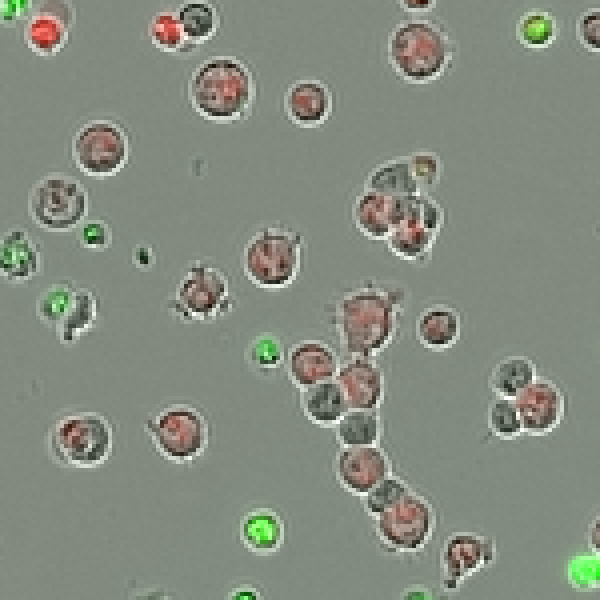
\includegraphics[width=.2\linewidth]{img/cluster_00.png}}}%
    \qquad
    \subfloat[$t=30$]{{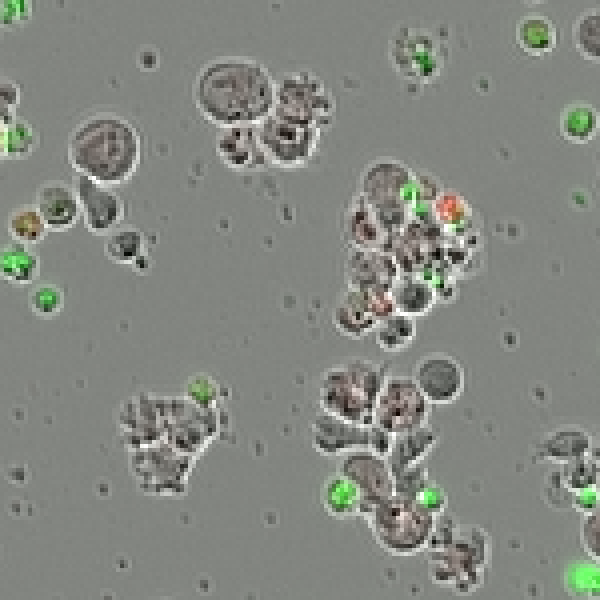
\includegraphics[width=.2\linewidth]{img/cluster_15.png}}}%
    \qquad
    \subfloat[$t=60$]{{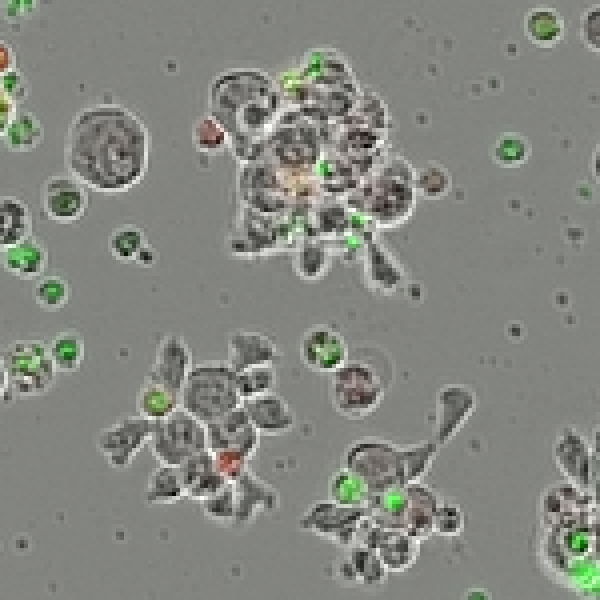
\includegraphics[width=.2\linewidth]{img/cluster_30.png}}}%
	\qquad
    \subfloat[$t=90$]{{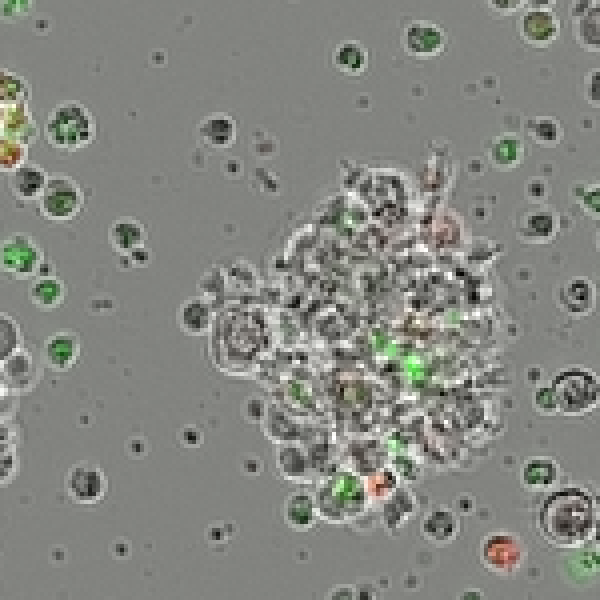
\includegraphics[width=.2\linewidth]{img/cluster_45.png}}}%
\caption{CAR-T cells (devoid of fluorescence) attack Raji B cells by latching onto Raji cell surface antigens and delivering cytotoxic chemicals. The induced lysis of the target Raji cells yields growing clusters of cellular matter.}
\label{fig:cluster_frames}
\end{figure}

%Phase contrast microscopy is a traditional microscopy technique developed in the 1930s that owes its popularity to both the simplicity of its experimental setup and a high contrast that is obtained by a smart arrangement of ring-shaped filters in the optical path. This high contrast, that does not require any particular sample preparation, allows to see structures in cells that are typically hidden in bright-field microscopy.
%
%In contrast, fluorescence microscopy allows to mark specific structures in cells with high contrast, either by immunofluorescence, live dyes or by genetic encoding of fluorescent reporters. Fluorescence microscopy is therefore the method of choice if we wish to highlight certain proteins of interest or the cellular compartments where these proteins localise. Importantly, this makes fluorescence microscopy particularly amenable for computational analysis. However, this high specificity and excellent contrast come at the price of visualising only partial information (only the marked proteins/cellular structures), of accepting a less physiological system (e.g. genetically modified cells) or more complicated experimental protocols (e.g. by the use of live dyes) and several experimental complications (such as fading dyes), in particular when imaging assays are performed over several days.

\subsection{Coping with fluorescent quenching}

Image-based screens of CAR-T cells, combining phase contrast and fluorescence microscopy, suffer from the gradual quenching of the fluorescent signal, making the reliable tracking of cell populations across time-lapse imagery difficult. We saw throughout Section \ref{subsec:phenomena} the diminished mCherry (red) fluorescent signal in latter time steps. In Figure \ref{fig:unnormalised_channels} we see how the distribution of total image fluorescence diminishes across time, regardless of well. Already, the quenching effect obfuscates the interpretation of the experiments by lab technicians. It is furthermore a complication for learning algorithms, as fluorescence becomes inversely correlated with the various cellular phenomena occurring in the latter stages of the experiment, for example: the dissemination of large cells due to cell growth, and the appearance of cell clusters due to mitosis, as illustrated above. Learning only on earlier frames, where the fluorescence is strongest, is unlikely to suffice. To mitigate the quenching effect, we normalise by,

\begin{equation}
x' = \min(1, \frac{\bar{x_0}}{\bar{x}}\cdot\frac{x - \min(x)}{\text{perc}_{99}(x) - \min(x)})
\end{equation}

where $\hat{x}_0$ and $\hat{x}$ are the means of the initial image and the image to be normalised, and $\text{perc}_{99}$ returns the $99$th percentile intensity. We then threshold by some small value $\tau$ to remove background noise.

\begin{figure}[h!]
\centering
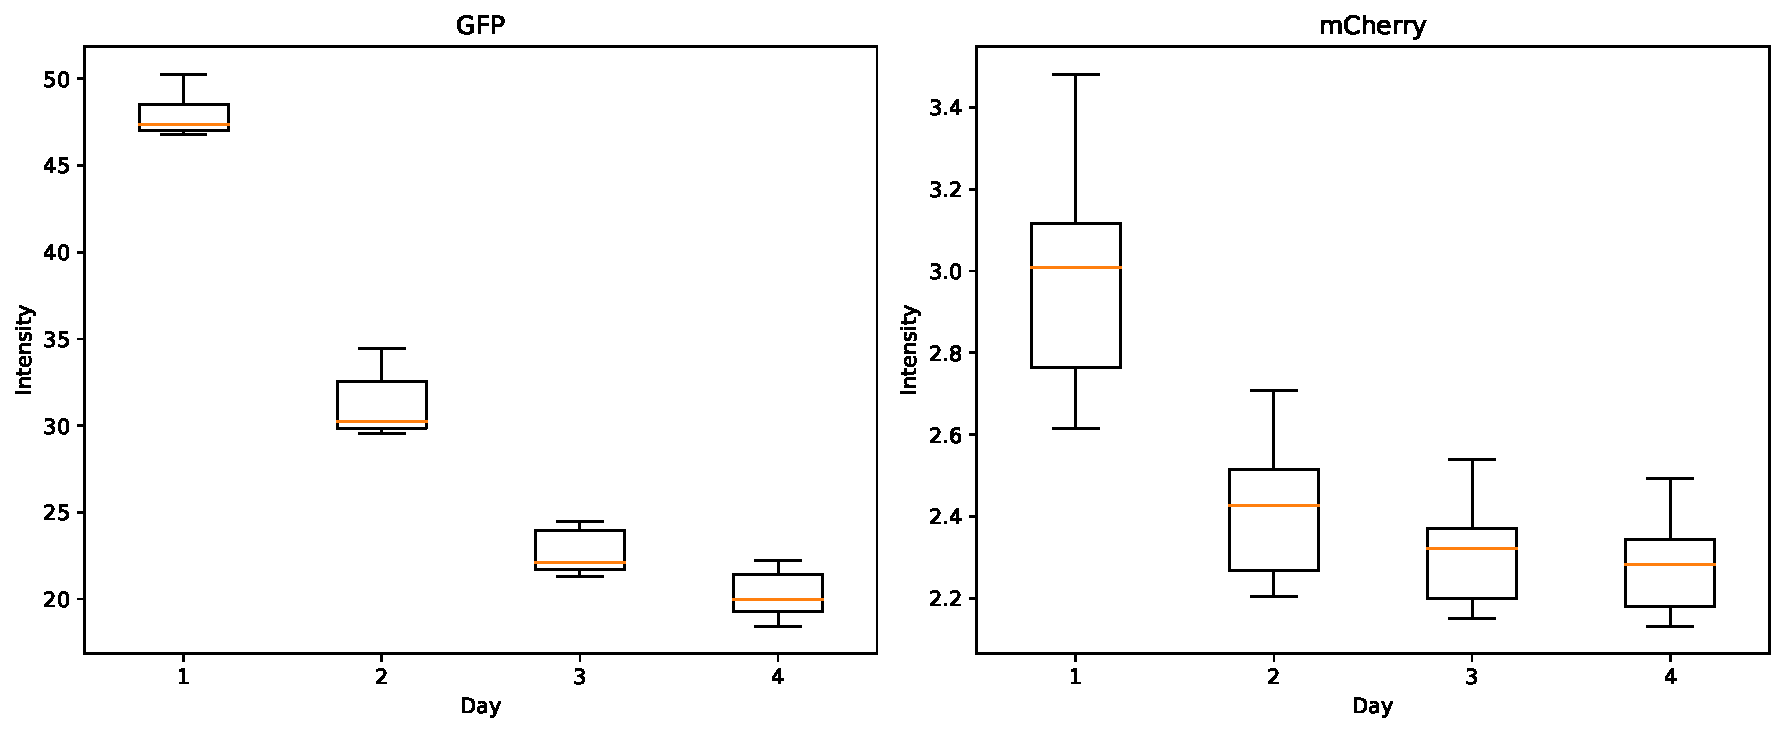
\includegraphics[width=0.85\textwidth]{img/unnormalised_channels.pdf}
\caption{Comparison of average GFP (left) and mCherry (right) fluorescence measured across at different fields of view and compared $24$ hour intervals. One may observe the quenching effect of fluorescence over time, which occurs most rapidly in the first increment.}
\label{fig:unnormalised_channels}
\end{figure}

%\begin{figure}[h!]
%\centering
%\includegraphics[width=\textwidth]{img/normalised_channels.pdf}
%\caption{Aligned image channel crops ($200 \times200$px) marking living Raji cells in mCherry (left), dead cells in GFP (center), and phase contrast (right).}
%\label{fig:gan_samples}
%\end{figure}

\section{Fluorescent labeling}
\label{sec:fluorescent_labeling}

In biological experiments pairing transmitted light and fluorescent signals, the fluorescence may often be largely inferred from the transmitted light image alone, as in \cite{christiansen2018silico}, \cite{ounkomol2018label}, and \cite{lee2018deephcs}. That is, given the pair $X, Y$ of transmitted light and fluorescent image, the fluorescent labeler $F$ learns a mapping such that,

\begin{equation}
F(X) \approx Y
\end{equation}

Note that the prospects for \emph{fluorescent labeling} will always depend on, among other things, the available image resolution. While \cite{ounkomol2018label} predicted fluorescent images of nucleoli, nuclear envelope, and microtubules from transmitted light images with a median Pearson correlation coefficient $r \geq 0.8$, ``painting'' other organelles such as desmosomes and Golgi apparatus worked far less well $r \leq 0.2$. In our experiments the relatively low resolution of cells must therefore by compensated by high-level morphological cues associating phenotype with fluorescence.

Here we present a family of models for performing fluorescence labeling of our phase contrast images automatically. The motivations of the system are twofold: firstly, it can be used as a visualisation tool; secondly, it may serve as an intermediate step in a cell counting system. Naturally, the quality of the latter function depends on that of the former.

\subsection{Image-to-image translation models}
\label{subsec:image_to_image}

Though not the only fluorescence labeler in the literature, we posit the ``F-Net'', proposed by \cite{ounkomol2018label}, to be the proper baseline for our problem, on the grounds that it is essentially a repurposed U-Net (\cite{ronneberger2015u}), a widely studied architecture. This architecture has a deep encoder-decoder structure, such as the autoencoders studied in Section \label{subsubsec:dimensionality_reduction}, albeit fully convolutional, and with \emph{skip connections} concatenating each upsampling layer with its opposite downsampling layers. We give provide the full architecture specification in Appendix \ref{appendix:fnet}. The network is trained against the objective function,

\begin{equation}
\min_F \mathcal{L}_{L_2}(F) = \mathbb{E}_{\mathbf{x} \sim p(\mathbf{x})}[||\mathbf{y} - F(\mathbf{x})||_2^2]
\label{eq:l2_loss}
\end{equation}

that is, to minimise the expectation of mean square error over the distribution of input images $\mathbf{x}$ and target images $\mathbf{y}$, where $F : \mathbf{x} \to \mathbf{y}$ is the labeler network parameterised by a set of weights $\theta$. In our use cases, the input images are the phase contrast images, and the target images are the fluorescent channels. By default, we train the network to predict a single fluorescent channel (as in \cite{ounkomol2018label}), although evidently, one could train a multi-task labeler to predict a multiplexed fluorescent output. Our experiments with this approach did not yield a significant improvement, however.

The F-Net approach is more or less generalised by the image-to-image translation models proposed in \cite{isola2017image}. Thus, we formulate the family of \texttt{pix2pix} models,

\begin{equation}
\min_G\max_D\mathcal{L}_{PIX}(D_{patch}, G) = \mathcal{L}_{cGAN}(D_{patch}, G) + \lambda\mathcal{L}_{1}(G)
\label{eq:pix2pix_loss}
\end{equation}

where $\mathcal{L}_{1}(G) = \mathbb{E}[||G(\mathbf{x}) - \mathbf{y}||_1]$ is mean absolute error with tuning hyperparameter $\lambda$ and $\mathcal{L}_{cGAN}$ is the conditional GAN (cGAN) objective,

\begin{align}\mathcal{L}_{cGAN}(D, G) = \mathbb{E}_{\mathbf{x} \sim p(\mathbf{x})}[\log D(\mathbf{x} | \mathbf{y})] + \mathbb{E}_{\mathbf{z} \sim p(\mathbf{z})}[\log(1 - D(G(\mathbf{z} | \mathbf{y})))]
\end{align}

where $D$ is the discriminator and $G$ is the generator, equivalent to $F$ in all ways aside from it using a hyperbolic tangent ($\tanh$) activation function, as is conventional for DCGANs, rather than a linear one. The variable $\mathbf{z}$ refers to the generator's noise input. In the image-to-image setting, the discriminator network is a fully-convolutional network denoted ``PatchGAN'' (see Appendix \ref{appendix:patch_gan}),

\begin{equation}
d_{patch} : X, Y \to [0, 1]^{h\times w}
\end{equation}

producing an $h\times w$ grid of outputs rather than a single neuron, with each grid element critiquing an overlapping region of the input image. The grid of outputs are then averaged to give the discriminator,

\begin{equation}
D_{patch}(\mathbf{x}, \mathbf{y}) = \frac{1}{hw}\sum_{i=0}^h\sum_{j=0}^w d_{patch}(\mathbf{x}, \mathbf{y})_{ij}
\end{equation}

In practice, the conditioning means inputs are concatenated channel-wise. \cite{isola2017image} make the extremely insightful observation, however, that a GAN learns its own loss function via the discriminator, which penalises ``unrealistic'' images. As such, it is an infinitely flexible methodology and the discriminator $D$ can be understood to act as an adaptive loss function, analagous to the way features are learned and optimised for the task of classification within the layers of a deep classifier. The choice of $L_1$ over an $L_2$ auxiliary loss is based on the empirical observation that $L_2$ leads to blurry results, something we observe presently. The \texttt{pix2pix} system has been demonstrated to be effective on a myriad of image-to-image translation problems. Just as with U-Net, they can achieve impressive results on a relatively small number of images.

In addition to the above, we also train the F-Net $F$ against a mean absolute error loss,

\begin{equation}
\min_F\mathcal{L}_{L_1}(F) = \lambda\mathcal{L}_{1}(F)
\label{eq:l1_loss}
\end{equation}

We trained all models (Equations \ref{eq:l2_loss}, \ref{eq:pix2pix_loss}, and \ref{eq:l1_loss}) on $1120$ non-overlapping $256\times256$px phase contrast crops selected from the first $14$ fields of view from the Raji-only experiments (row A of the plate). The cropping strategy sampled from the first frame of each $24$-hour window, for the first $96$ hours of each time lapse movie. This strategy was adopted to maximise the available variation in the training data, without losing too much to the fluorescent quenching effect of later frames, while at the same time retaining the convenience of keeping all images in memory.   Validation and testing was performed according to the same strategy on independent fields A06\_03 and A06\_04. Batches of size $1$ were sampled randomly and all models were trained with the Adam optimiser with $(\beta_0, \beta_1) = (0.5, 0.999)$ and maximum learning rate $2\times10^{-4}$.

\subsection{Results}

In practice, a fluorescence prediction can be considered accurate if the placement of its predictions are accurate, even if it does not match the ground truth intensities accurately. For this reason \cite{ounkomol2018label} propose evaluating based on the Pearson correlation coefficient (PCC),

\begin{align}
r = \frac{\sum (x - \bar{x})(y - \bar{y})}{\sqrt{\sum (x - \bar{x})^2\sum (y - \bar{y})^2}}
\end{align}

over all pixels $x$ in the prediction and $y$ in the test image. We compare the average PCC correlation across all test images for each of the three models and each mode (GFP, mCherry) (see Figure \ref{fig:pix2pix_pcc}). The best overall performance comes from the $L_2$ model with mean $0.7617$ and standard deviation $0.1049$ for mCherry labeling, and mean $0.6163$ and standard deviation $0.0931$ for GFP. The pix2pix system performs at mean $0.7573$ and standard deviation $0.0814$ for mCherry, and mean $0.5848$ and standard deviation $0.0972$ for GFP. Finally, the $L_1$ models performs at mean $0.7720$ and standard deviation $0.0727$ for mCherry, and $0.5115$ and standard deviation $0.1099$ for GFP. Paradoxically, the $L_2$ model appears, by inspection, to generate worse results, with a significant amount of fluorescent ``spillage'' and blur effects. However, this noise can be removed with a simple thresholding operation. The pix2pix outputs look immediately sharper, but ultimately fail more often to apply fluorescence where it counts, leading to more false negatives. On the other hand, it is also clear that the $L_2$ and $L_1$ models exhibit a greater degree of mode collapse than the pix2pix model, which necessarily varies its fluorescent labeling to continuously fool the discriminator.

%\begin{figure}[h!]
%\centering
%\includegraphics[width=0.65\textwidth]{img/pix2pix_mse.pdf}
%\caption{Aligned image channel crops ($200 \times200$px) marking living Raji cells in mCherry (left), dead cells in GFP (center), and phase contrast (right).}
%\label{fig:unnormalised_channels}
%\end{figure}

\begin{figure}[h!]
\centering
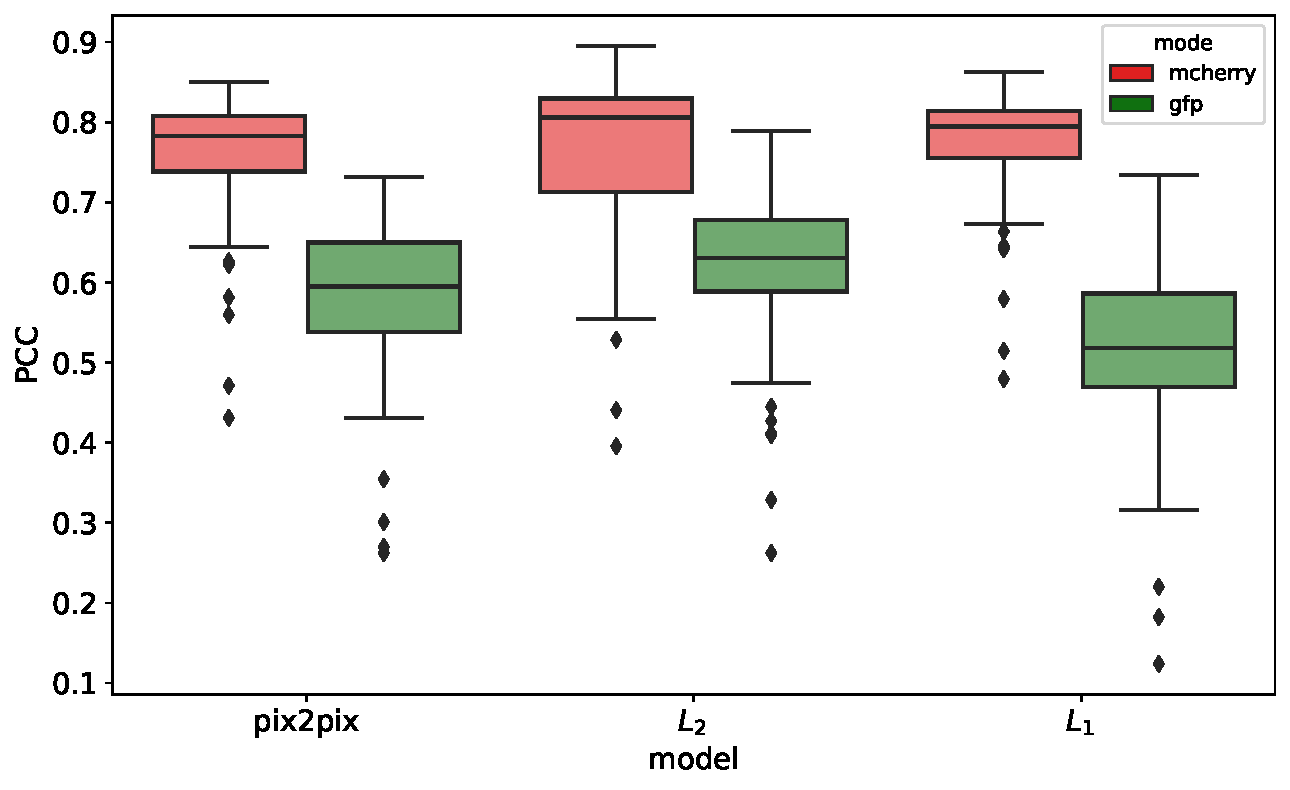
\includegraphics[width=0.65\textwidth]{img/pix2pix_pcc.pdf}
\caption{Pearson correlation coefficients for outputs of three fluorescent labelers, for both mCherry and GFP fluorescence prediction, measured over $80$ test images.}
\label{fig:pix2pix_pcc}
\end{figure}

\subsubsection{Full fluorescence outputs}

An important qualitative test is to visualise the joint model outputs in full fluorescent colour, as well as in time lapse. To produce an appealing output, we first correct for a ``camera shake'' effect of the plate moving inside the microscope. Between successive frames, this is usually no more than $10 \mu m$, corresponding to about $7$px, in any direction. We therefore find the necessary correction $(\delta x, \delta y)$ frame by frame by brute force over a suitable range of offsets. Fortunately, the Raji cells do not move much over time, and we can therefore find the right offset as the one that minimises the squared error between the frames. The images are each cropped slightly to account for the extents of the cumulative displacements in each direction caused by the shake. This tends to be a small amount, apparently with the camera displacements occurring around a fixed center of mass. Lastly, we correct the frames of the fluorescent channels by the same offsets discovered in the phase contrast.

We set RGB pixel at position $(i, j)$ of each full fluorescence image $I$ as,

\begin{equation}
I_{ij} = [M_{ij} + P_{ij}, G_{ij} + P_{ij}, P_{ij}]
\end{equation}

where $M$ is the mCherry channel, $G$ is the GFP channel, and $P$ is the phase contrast image. The values are further clipped to the range $[0, 1]$. In Figures \ref{fig:full_colour_raji} and \ref{fig:full_colour_t_cells} we compare synthesised images combined from the respective fluorescent labelers to the corresponding ground truth fluorescence. The errors are manifest, yet the \texttt{pix2pix} models do a fine job of discerning cell types, implicit in its application of GFP over dead Raji cells in the Raji-only experiment (Figure \ref{fig:full_colour_raji}) and its leaving T cells unlabelled in the full CAR-T experiment \ref{fig:full_colour_t_cells}, as per the logic of Equation \ref{eq:fuzzy_logic}. The predicted fluorescence intensity levels also closely approximate those of the ground truth. Nevertheless, it should be noted that the the mutual information between fluorescence intensity and phase contrast morphology may ultimately be too small to always guarantee an accurate prediction of intensity. For this reason, we must accept, for example, that certain dead cells appear more yellow than green, and vice versa. One possible extension of our work would be to incorporate time information into the prediction, which might alleviate this effect. Ultimately, however, we can confirm that for the broader picture, the fluorescent labeling is a success as a visualisation tool, at least for the earlier frames of the video, and we should ought now to consider how to incorporate it into a practicable tool for the experimental setting.

We release full $110$-frame time lapse movies comparing prediction (left) and ground truth full fluorescence (right) online: Raji-only $256\times256$px\footnote{https://jcboyd.github.io/assets/car-t-videos/raji\_target/256.mp4}, Raji-only $512\times512$px\footnote{https://jcboyd.github.io/assets/car-t-videos/raji\_target/512.mp4}, full CAR-T $256\times256$px\footnote{https://jcboyd.github.io/assets/car-t-videos/CAR\_June/256.mp4}, and full CAR-T $512\times512$px\footnote{https://jcboyd.github.io/assets/car-t-videos/CAR\_June/512.mp4}.

\begin{figure}%
    \centering
    \subfloat[Prediction ($t = 0$)]{{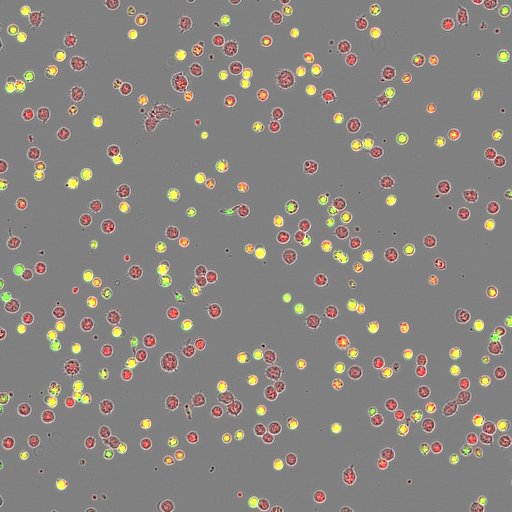
\includegraphics[width=.45\linewidth]{img/full_colour_0001a.png}}}%
    \qquad
    \subfloat[Ground truth ($t = 0$)]{{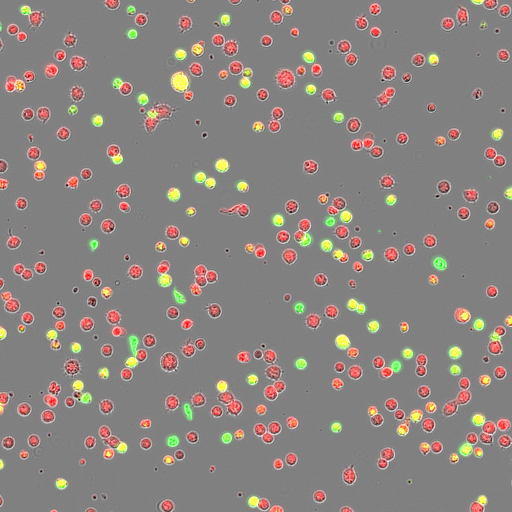
\includegraphics[width=.45\linewidth]{img/full_colour_0001b.png}}}%
    \qquad
    \subfloat[Prediction ($t = 48$)]{{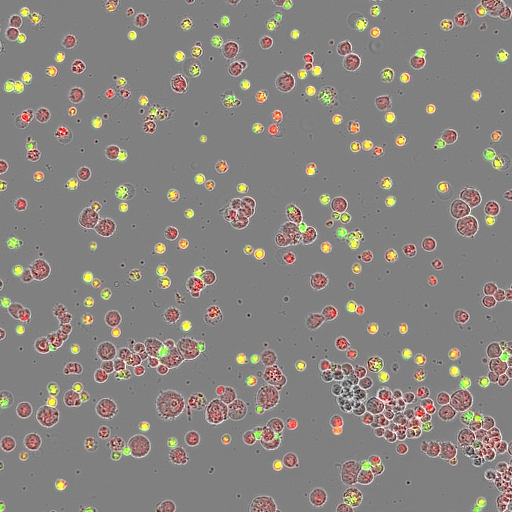
\includegraphics[width=.45\linewidth]{img/full_colour_0048a.png}}}%
    \qquad
    \subfloat[Ground truth ($t = 48$)]{{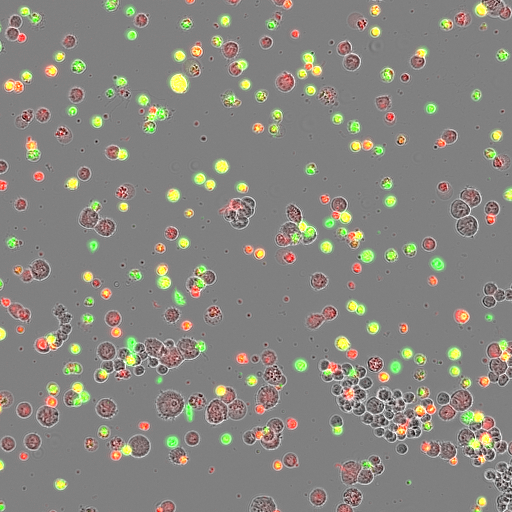
\includegraphics[width=.45\linewidth]{img/full_colour_0048b.png}}}%
\caption{Full fluorescence for indicative ($512 \times 512$px) crop from an Raji-only experiment. Columns distinguish fluorescent labeler predictions (left) and ground truth (right); rows distinguish times an early frame ($t=0$) (top) and a later one ($t=48$) (bottom).}
\label{fig:full_colour_raji}
\end{figure}

\begin{figure}%
    \centering
    \subfloat[Prediction ($t = 0$)]{{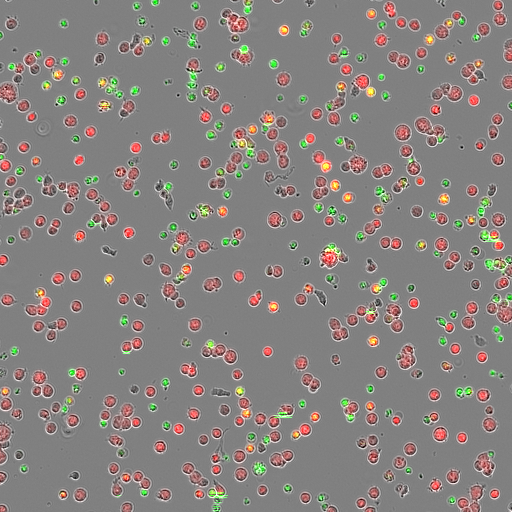
\includegraphics[width=.45\linewidth]{img/full_colour_t_0000a.png}}}%
    \qquad
    \subfloat[Ground truth ($t = 0$)]{{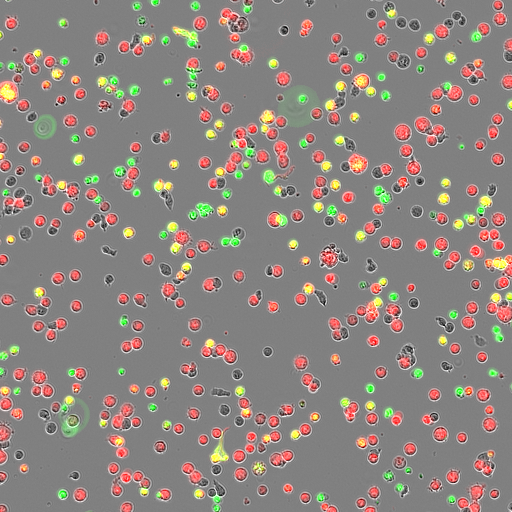
\includegraphics[width=.45\linewidth]{img/full_colour_t_0000b.png}}}%
    \qquad
    \subfloat[Prediction ($t = 40$)]{{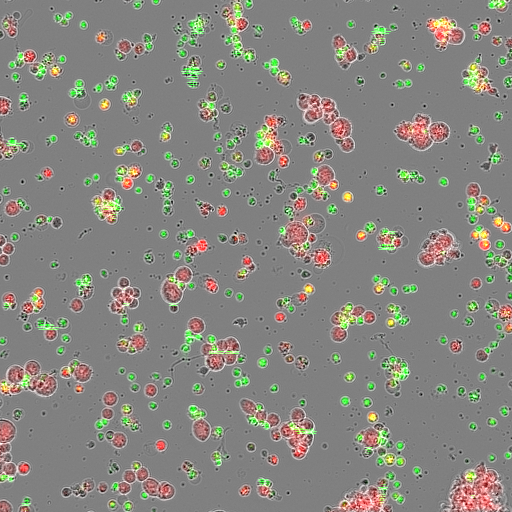
\includegraphics[width=.45\linewidth]{img/full_colour_t_0040a.png}}}%
    \qquad
    \subfloat[Ground truth ($t = 40$)]{{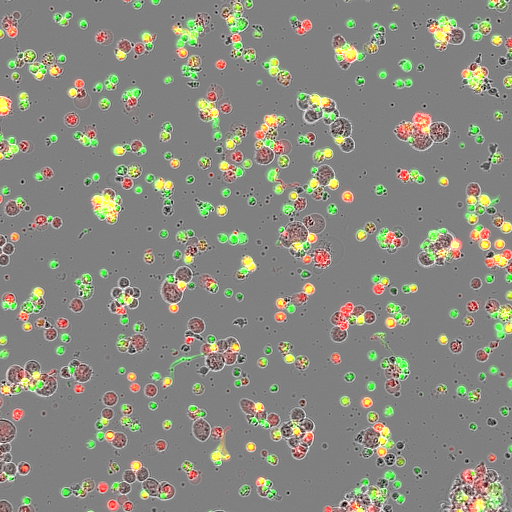
\includegraphics[width=.45\linewidth]{img/full_colour_t_0040b.png}}}%
\caption{Full fluorescence for indicative ($512 \times 512$px) crop from a CAR-T experiment. Columns distinguish fluorescent labeler predictions (left) and ground truth (right); rows distinguish times an early frame ($t=0$) (top) and a later one ($t=40$) (bottom).}
\label{fig:full_colour_t_cells}
\end{figure}

%\begin{figure}%
%    \centering
%
%\caption{Put your caption here}
%\label{fig:full_colour_0048}
%\end{figure}

%\begin{figure}[ht]
%\begin{subfigure}{.5\textwidth}
%  \centering
%  % include first image
%  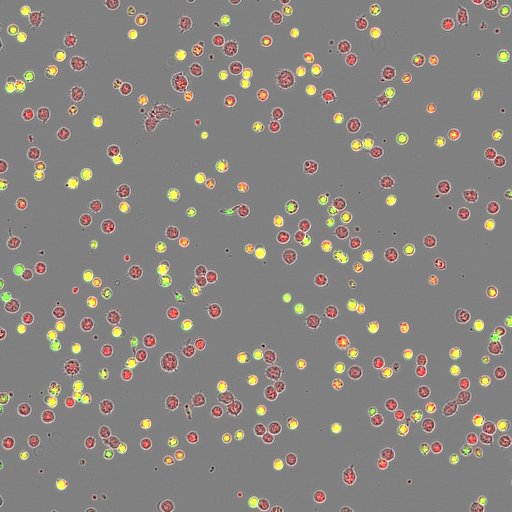
\includegraphics[width=.8\linewidth]{img/full_colour_0001a.png}  
%  \caption{Put your sub-caption here}
%  \label{fig:sub-first}
%\end{subfigure}
%\begin{subfigure}{.5\textwidth}
%  \centering
%  % include second image
%  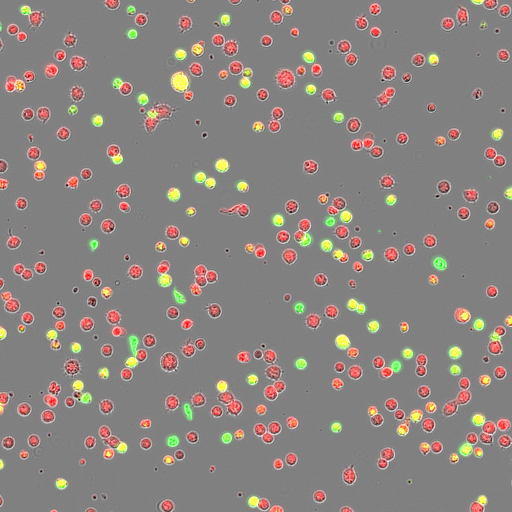
\includegraphics[width=.8\linewidth]{img/full_colour_0001b.png}  
%  \caption{Put your sub-caption here}
%  \label{fig:sub-second}
%\end{subfigure}
%\caption{Put your caption here}
%\label{fig:full_colour_0001}
%\end{figure}
%
%\begin{figure}[ht]
%\begin{subfigure}{.5\textwidth}
%  \centering
%  % include first image
%  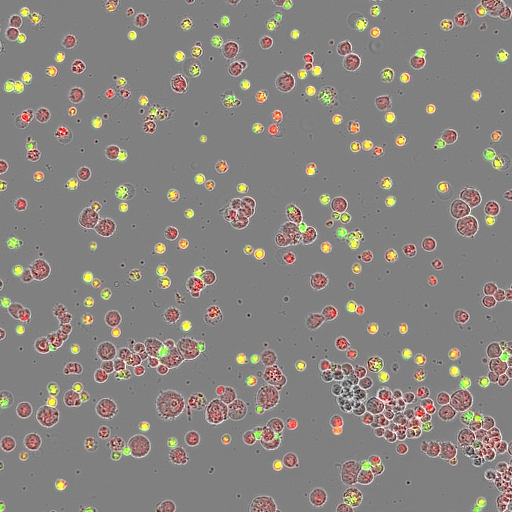
\includegraphics[width=.8\linewidth]{img/full_colour_0048a.png}  
%  \caption{Put your sub-caption here}
%  \label{fig:sub-first}
%\end{subfigure}
%\begin{subfigure}{.5\textwidth}
%  \centering
%  % include second image
%  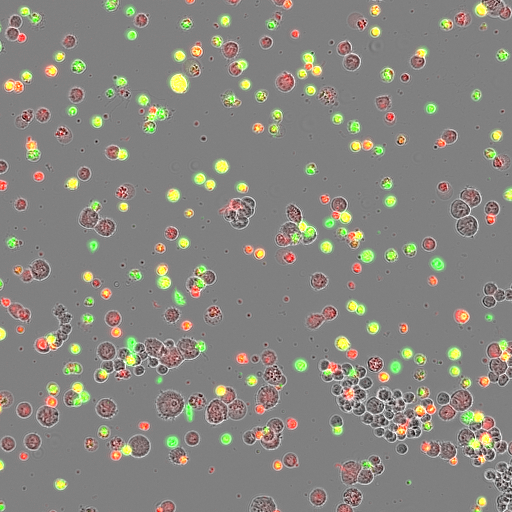
\includegraphics[width=.8\linewidth]{img/full_colour_0048b.png}  
%  \caption{Put your sub-caption here}
%  \label{fig:sub-second}
%\end{subfigure}
%\caption{Put your caption here}
%\label{fig:full_colour_0048}
%\end{figure}

\subsection{Bridging the gap to cell detection}

In our problem context, we would like to derive a quantitative profile from live cell imaging data. While effective as a visualisation tool, fluorescent labeling only goes partway towards a full quantification of the phase contrast contents. Consider sample outputs for densely clustering cells, given in Figure \ref{fig:in_silico_problems}. Here we can see how the task of counting cells is far from over following fluorescent labeling, with dense ``clouds'' of fluorescence corresponding to masses of cells. One can imagine all sorts of \emph{post hoc} solutions for disambiguating these fluorescent clouds.

\begin{figure}%
    \centering
    \subfloat[Phase contrast input]{{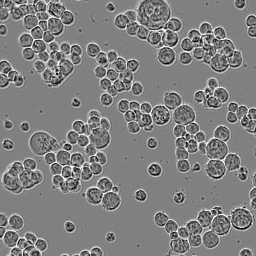
\includegraphics[width=.45\linewidth]{img/example_1_pc.png}}}%
    \qquad
    \subfloat[mCherry fluorescent output]{{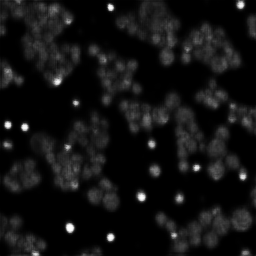
\includegraphics[width=.45\linewidth]{img/example_1_mcherry.png}}}%
    \qquad
    \subfloat[Phase contrast input]{{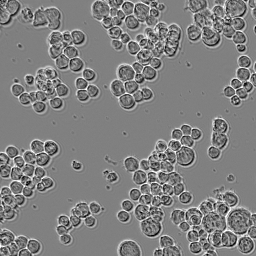
\includegraphics[width=.45\linewidth]{img/example_2_pc.png}}}%
    \qquad
    \subfloat[mCherry fluorescent output]{{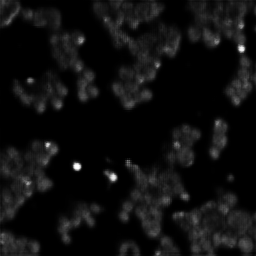
\includegraphics[width=.45\linewidth]{img/example_2_mcherry.png}}}%
\caption{Fluorescent labeler outputs produce dense clouds of mCherry fluorescence for two manually selected phase contrast inputs. These outputs may be difficult to disambiguate.}
\label{fig:in_silico_problems}
\end{figure}

\subsubsection{Blob detection for disambiguating fluorescent labels}

As Raji cells have a consistent size and simply, circular geometry, one approach to counting individual cells from the fluorescent label outputs is with \emph{blob detection}. A simple approach to blob detection is with a Laplacian of Gaussian (LoG) filter. That is,

$$\Delta G_\sigma(x, y) * f(x, y) = [\nabla_{xx}G_\sigma(x, y) + \nabla_{yy}G_\sigma(x, y)] * f(x, y)$$

where $\Delta$ is the Laplacian operator (sum of second partial derivatives), $G_\sigma$ is a Gaussian filter with standard deviation $\sigma$ and $f$ is an image. Blobs distribute intensities in a Gaussian-like way, and the Gaussian pre-filter smooths the image. The second derivative of a Gaussian has a minimum in the center of bell curve, thus marking the center of the blob. The maxima detected in the resultant image are the detected blobs. Usually the filter is performed over a range of scales, with the maxima taken over the z-stack.

In practice, the tunable parameters for LoG blob detection are the range of standard deviations $\{\sigma_i\}$ to test for (corresponding to the anticipated size range) and a threshold $\theta$ on the minimum permissible intensity. These we tune by hand. We provide an example of this approach to blob detection of fluorescent outputs in Figure \ref{fig:blob_detection}.

We find, however, that this simple approach to blob detection does not suffice for cases such as in in Figure \ref{fig:in_silico_problems}. While some system could surely be devised to infer the number of cells from a mass of flouroscence, in the following section we study an alternative approach based on the fundamentally distinct methodology of object detection, which makes counting cells a primary objective.

\section{Object detection system}
\label{sec:object_detection_system}

\emph{This section contains an extended version of a paper published in at the International Symposium for Biomedical Imaging in 2020.}

We found in the previous section a limitation on the scope of fluorescent labeling for counting cells. This brings us back to a more conventional high content analysis (HCA). Whereas in Chapter \ref{Chapter3} we were concerned with generating a phenotypic profile that characterised a drug effect effectively, regardless of how obscure the meaning of the profile elements. In the present context, we are concerned with the more comprehensible task of counting cell types in time. Note that this task conforms to the conventional pipeline (see Section \ref{subsec:hca}). In particular, the dimensionality reduction step will be fulfilled by the attribution of a cell type,

\begin{equation}
\mathbf{z} = f(\mathbf{x})
\end{equation}

where $\mathbf{z} \in \{0, 1\}^K$ and $\sum_{k=0}^K z_k = 1$ for $K$ the number of cell classes, that is, $\mathbf{z}$ is one-hot, for extracted cell features $\mathbf{x}$, and cell classifier $f$. The cell population is then summarised by aggregation as a simple summation or average, giving the number or proportion of cells per cell class respectively in the phenotypic profile,

\begin{equation}
\mathbf{p} = \frac{1}{N}\sum_{i=1}^N f(\mathbf{x}_i)
\end{equation}

As we shall see, the first three stages of the HCA pipeline are achieved by a single neural network.

A phenotypic profile of this nature summarises a single image frame. However, we are interested in summarising a full time lapse movie. Therefore, our aim is to create a set of such count profiles,

\begin{equation}
\mathbb{P} = \{\mathbf{p}_i\}_{i=0}^{T},
\end{equation}

where $\mathbf{p}_i \in \mathbb{R}^K$ for $K$ classes is the $i$th profile in a series of $T$ frames. This ordered set amounts to a set of $K$ time series, one per class, of length $T$, and is our final output in Section \ref{subsec:results}.

In Section \ref{subsec:data} we describe an acquisition and preprocessing pipeline for an experimentally-generated object detection ground truth with which to train our object system. In Section \ref{subsec:training} we specify this system, and in Section \ref{subsec:results} we describe our evaluation methodology and report model performance on two manually annotated datasets. In this Section we consider only the Raji-only experimental setting. Note that our methodology should naturally extend to other the full CAR-T setting also, something we intend to address in future work.

\subsection{Experimentally-generated ground truth}
\label{subsec:data}

Our pipeline (see Figure \ref{fig:pipeline_ground_truth}) begins by applying a Gaussian filter (tuned to $\sigma = 2$) to the phase contrast image. We then segment cells by subtracting a background image formed with a mean filter of diameter $19$px, before clipping to zero as in \cite{walter2010automatic}. We fill object holes with a morphological reconstruction by erosion and use a morphological opening to remove small details. An example of this pipeline depicted in Figure \ref{fig:ground_truth_pipeline_example}. We further filter objects outside a reasonable size range ($< 6 \times 6$px $\approx 50 \mu m^2$, determined by ranking cell areas), as these tend to be dust and other non-cellular particles on the well surface. An Otsu threshold on the distribution of averaged GFP signal per cell is then used to allocate a class (living/dead) for each connected component (see Figure \ref{fig:gfp_bimodal}. To train our object detector (Section \ref{subsec:training}), we also randomly sample background crops from the images, allowing for partial overlaps with cells.

\tikzstyle{block} = [rectangle, draw, fill=blue!20, node distance=2.5cm,
    text width=3.5em, text centered, rounded corners, minimum height=3em]
\tikzstyle{line} = [draw, -latex']

\begin{figure}
\centering
\begin{tikzpicture}[node distance=0.5cm, text width=3em, minimum height=3em, font=\tiny]
    % Place nodes
    \node [block, fill=red!20] (green) {GFP};
    \node [block, left of=green, fill=red!20] (pc) {Phase contrast};
    \node [block, right of=green, fill=red!20] (red) {mCherry};

	\node [block, below of=green] (fill) {Fill holes};
	\node [block, left of=fill] (bs) {Background subtraction};
	\node [block, left of=bs] (prefilter) {Prefilter};
	\node [block, right of=fill] (features) {Extract features};
	\node [block, right of=features] (classes) {Assign classes};
    % Draw edges
    \path [line] (pc) -- (prefilter);
    \path [line] (prefilter) -- (bs);
    \path [line] (bs) -- (fill);
	\path [line] (fill) -- (features);
%    \path [line] (fill) -- (label);
%    \path [line] (label) -- (features);
    \path [line] (features) -- (classes);
	\path [line] (green) -- (features);
	\path [line] (red) -- (features);
\end{tikzpicture}
\caption{Pipeline for automatic construction of ground truth for training object detection system. Basic image processing steps indicated in blue; image inputs indicated in red.}
\label{fig:pipeline_ground_truth}
\end{figure}

\begin{figure}[htb]
\centering
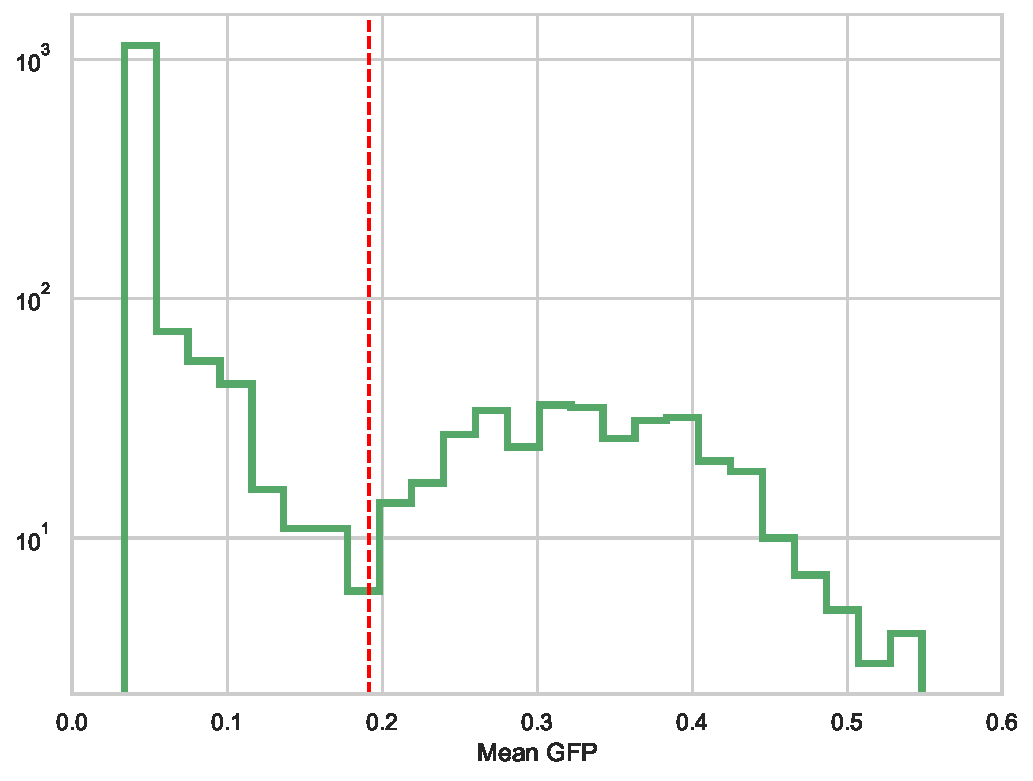
\includegraphics[width=0.85\textwidth]{img/gfp_bimodal.pdf}
\caption{Living and dead Raji cells revealed as distinct modes of a bimodal distribution on mean GFP fluorescence intensity per connected component of cell segmentation output.}
\label{fig:gfp_bimodal}
\end{figure}

\subsection{Object detection system}
\label{subsec:training}

In order to track cell phenotype populations over time, we require a robust object detection system to identify individual cells. The core of our system is a convolutional neural network and is detailed below.

\tikzstyle{block} = [rectangle, draw, fill=blue!20, node distance=2.5cm,
    text width=3.5em, text centered, rounded corners, minimum height=3em]
\tikzstyle{line} = [draw, -latex']

\begin{figure}
\centering
\begin{tikzpicture}[node distance=0.5cm, text width=3em, minimum height=3em, font=\tiny]
    % Place nodes
    \node [block, fill=red!20] (data) {Train data $(24\times24)$};
    \node [block, below of=data] (training) {Model training};
    \node [block, left of=training, fill=red!20] (architecture) {FCN architecture};
    \node [block, right of=training, fill=red!20] (classifier) {FCN classifier};
    \node [block, right of=classifier] (inference) {Model inference};
    \node [block, above of=inference, fill=red!20] (test) {Test data $(? \times ?)$};
    \node [block, right of=inference, fill=red!20] (probabilities) {Probability map};
    \node [block, below of=probabilities] (nms) {Non-maximum supp.};
    \node [block, below of=nms, fill=red!20] (bbs) {Bounding box proposals};
%    \node [block, above right of=cluster] (visualise) {Visualise t-SNE};
%    \node [block, below right of=cluster] (crops) {Sample crops};
    % Draw edges
    \path [line] (data) -- (training);
    \path [line] (architecture) -- (training);
    \path [line] (training) -- (classifier);
    \path [line] (classifier) -- (inference);
    \path [line] (test) -- (inference);
    \path [line] (inference) -- (probabilities);
    \path [line] (probabilities) -- (nms);
    \path [line] (nms) -- (bbs);
%    \path [line] (probabilities) -- (visualise);
%    \path [line] (cluster) -- (crops);
\end{tikzpicture}
\caption{Pipeline for training a deployment of a fully convolutional classifier. Training may occur on fixed-sized input ($24 \times 24$)px, but convolutions permit variable-sized inference.}
\end{figure}
%
%In this section we detail our object detection system and our pre- and post-processing methodology. All code for our system is publicly available\footnote{\texttt{https://github.com/jcboyd/tracking-lymphocytes}}.

\subsubsection{Training as a classifier}

Our preprocessing pipeline is imperfect and does not give a complete annotation of the cell populations as would be required by state-of-the-art detection systems such as \cite{redmon2016you}. We therefore opt for crop-wise training, where the bounding boxes of successfully segmented cells are padded, to create $24\times24$px crops, centered on the cells. Due to the low image resolution, we found this sizing provided sufficient contextual information to the network. Combined with background crops, this amounts to approximately 100,000 training examples in three classes. Samples are given in Figure \ref{fig:crops}.

\begin{figure}[htb]
\centering
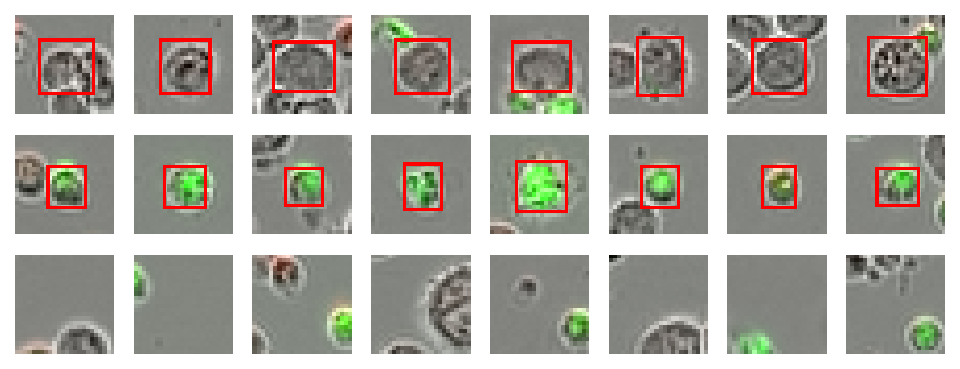
\includegraphics[width=\textwidth]{img/crops.pdf}
\caption{Samples of living Raji cells (top), dead cells (middle), background (bottom) annotated with bounding boxes. Fluorescence is included for clarity only and is not used in training.}
\label{fig:crops}
\end{figure}

% the following design: two consecutive blocks of $3\times3$ convolution $\to$ batch norm $\to$ ReLU activation; a $2 \times 2$ max pooling; two further blocks of $3\times3$ convolution $\to$ batch norm $\to$ ReLU activation; a final $1\times1$ convolutional layer with softmax activation.

Our network architecture is detailed in Table \ref{table:nn}. All weighted layers have a ReLU activation, except Output$_o$ and Output$_c$, which have softmax activations, and Output$_b$, which remains linear. The convolutions are all valid, and a $24\times24$px input image is reduced to $1\times1$px by the final layer. We implement this network in the \texttt{Keras} deep learning framework\cite{chollet2015keras} and all code for our system is publicly available\footnote{\texttt{https://github.com/jcboyd/detecting-lymphocytes}}. We train the network with stochastic gradient descent with learning rate $5 \times 10^{-3}$ and Nesterov momentum $(\mu = 0.9)$. Mini-batches of size 128 are sampled stochastically and simple data augmentation (horizontal and vertical flipping) is performed on the fly. We regularise the network with batch normalisation \cite{ioffe2015batch} and weight decay ($\lambda = 3 \times 10^{-5}$).

\begin{table}[ht!]
\begin{center}
\begin{tabular}{|c|c|c|c|}
\hline
Layer & Connection & Size & Output ($w \times h \times d$) \\
\hline
Input & - & - & $24 \times 24 \times 1$\\
\hline
Conv$_1$ & Input & ${3\times 3}$ & $22 \times 22 \times 16$  \\
Conv$_2$ & Conv$_1$ & ${3\times 3}$ & $20 \times 20 \times 16$ \\
MaxPool$_1$ & Conv$_2$ & ${2\times 2}$ & $10 \times 10 \times 16$ \\
Conv$_3$ & MaxPool$_1$ & ${3\times 3}$ & $8 \times 8 \times 64$ \\
Conv$_4$ & Conv$_3$ & ${3\times 3}$ & $6 \times 6 \times 64$ \\
MaxPool$_2$ & Conv$_4$ & ${2\times 2}$ & $3 \times 3 \times 64$ \\
Conv$_5$ & MaxPool$_2$ & ${1\times 1}$ & $1 \times 1 \times 128$ \\
Conv$_6$ & Conv$_5$ & ${1\times 1}$ & $1 \times 1 \times 128$ \\
\hline
Output$_o$ & Conv$_6$ & ${1\times 1}$ & $1 \times 1 \times 1$ \\
Output$_c$ & Conv$_6$ & ${1\times 1}$ & $1 \times 1 \times 1$ \\
Output$_b$ & Conv$_6$ & ${1\times 1}$ & $1 \times 1 \times 2$ \\
\hline
\end{tabular}
\end{center}
\caption{Specification of the network architecture. We distinguish three multitask outputs.}
\label{table:nn}
\end{table}

Inspired by \cite{redmon2016you}, we formulate a multi-task prediction in which we predict $Pr(o)$, where $o$ indicates the presence of an object in the center of the receptive field and, separately, $Pr(c | o)$, that is, the probability of cell phenotype class $c$ given the presence of an object. These probabilities are combined at inference time (Section \ref{subsubsec:inference}). In addition, our network performs regression on the height $h$ and width $w$ of the bounding box of the cell, measured as a fraction of the crop size from the crop centre. This information is readily available when generating the training set. Note that we make the assumption that our chosen crop size represents a hard maximum on the size of a cell's bounding box, a reasonable simplification for our dataset. Our network is therefore trained to minimise the loss function,

\begin{align}
\mathcal{L}(\mathbf{x}_i, o_i, c_i, w_i, h_i;\theta) = l_{o}(\hat{o}_i, o_i) &+ \mathbbm{1}_{o}^{i}\big[l_{c}(\hat{c}_i, c_i)\big] + \mathbbm{1}_{o}^{i}\big[l_{b}(\hat{w}_i, w_i, \hat{h}_i, h_i)\big]
\end{align}

with respect to model parameters $\theta$, where $l_{o}$ and $l_{c}$ are each a standard cross entropy and $l_b(\hat{w}_i, w_i, \hat{h}_i, h_i) = (\hat{w}_i - w_i)^2 + (\hat{h}_i - h_i)^2$. The estimates $\hat{o}_i, \hat{c}_i$ $\hat{w}_i$, and $\hat{h}_i$ are the network outputs for object presence, object class, and bounding box width and height. The indicator function $\mathbbm{1}_o^i = 1$ when training example $\mathbf{x}_i$ contains an object and $\mathbbm{1}_o^i = 0$ otherwise.

We benchmarked our network as a classifier of cropped cells against a logistic regression trained on features extracted from a pre-trained 50-layer ResNet\cite{he2016deep}. In order to do this, we resized our cropped cells to $32 \times 32$px and recorded the final convolutional layer of the ResNet, a vector of dimension $2048$. This baseline achieved an accuracy of $0.83$ on balanced test data, whereas our own network achieved $0.96$. Though deep pre-trained networks are known to be powerful general-purpose feature extractors\cite{sharif2014cnn}, they may also be over-parameterised for many problems\cite{raghu2019transfusion}.
%It does appear, however, the two cell classes are not perfectly separable. This can be due to the imperfections of our ground truth generation, but also that the transmitted light image may not convey the full biological information of the fluorescent signal, as discussed in \cite{ounkomol2018label}.

\subsubsection{Inference as a detector}
\label{subsubsec:inference}

%\begin{figure*}[t!]
%\includegraphics[width=\textwidth]{img/nms.pdf}
%\caption{The processing of a test image. Row-wise then column-wise: phase contrast input image; raw model bounding box predictions; non-maximum suppression post-processing; finally, for comparison, the corresponding full fluorescence image.}
%\label{fig:nms}
%\end{figure*}

\begin{figure}%
    \centering
    \subfloat[]{{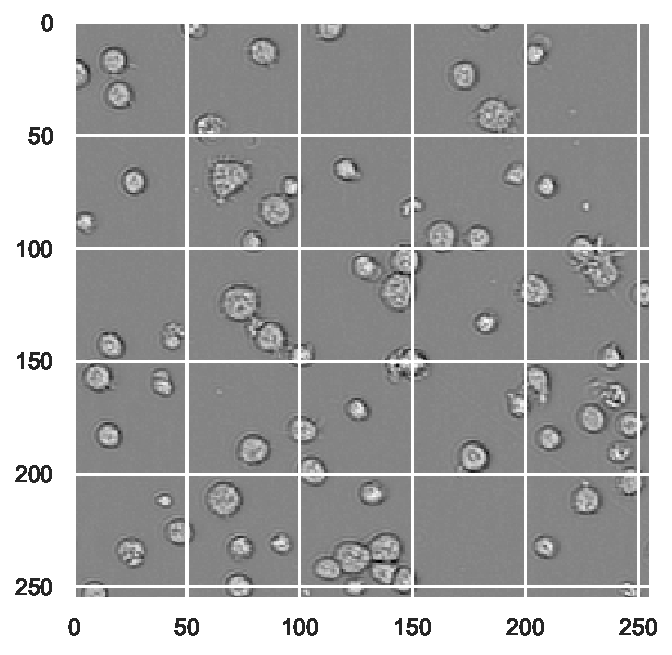
\includegraphics[width=.45\linewidth]{img/nms_input.pdf}}}%
    \qquad
    \subfloat[]{{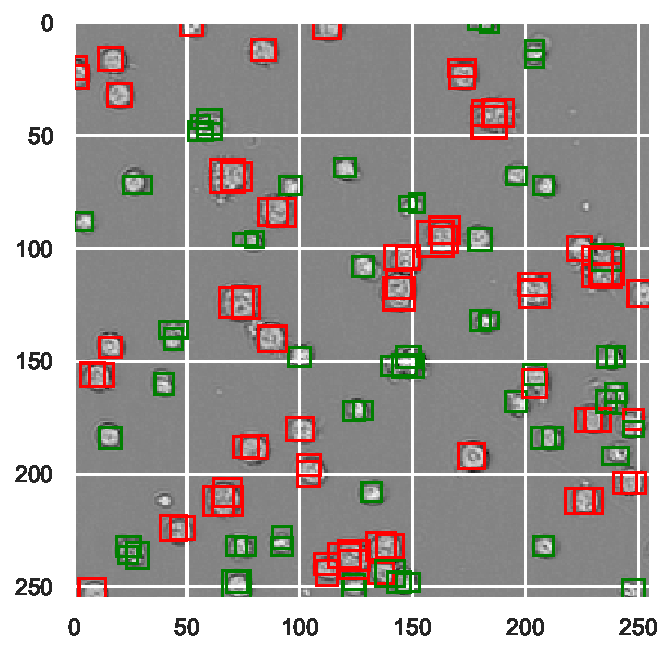
\includegraphics[width=.45\linewidth]{img/nms_raw_detections.pdf}}}%
    \qquad
    \subfloat[]{{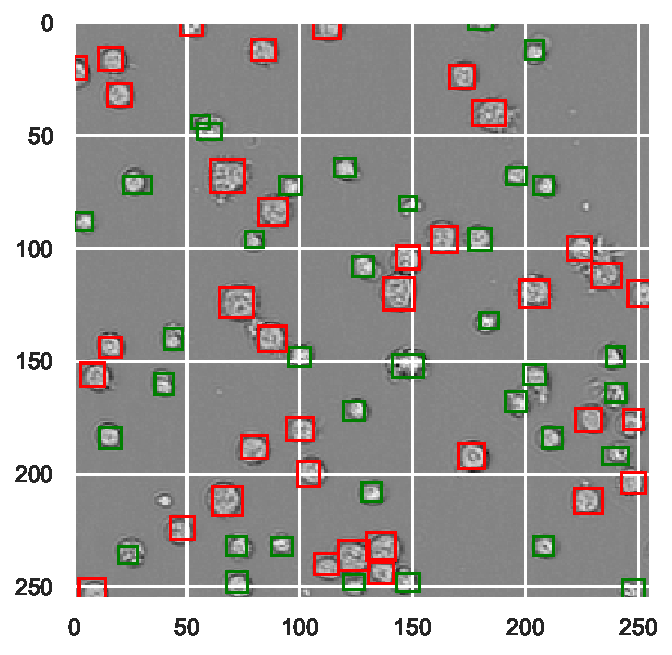
\includegraphics[width=.45\linewidth]{img/nms_post_nms_detections.pdf}}}%
    \qquad
    \subfloat[]{{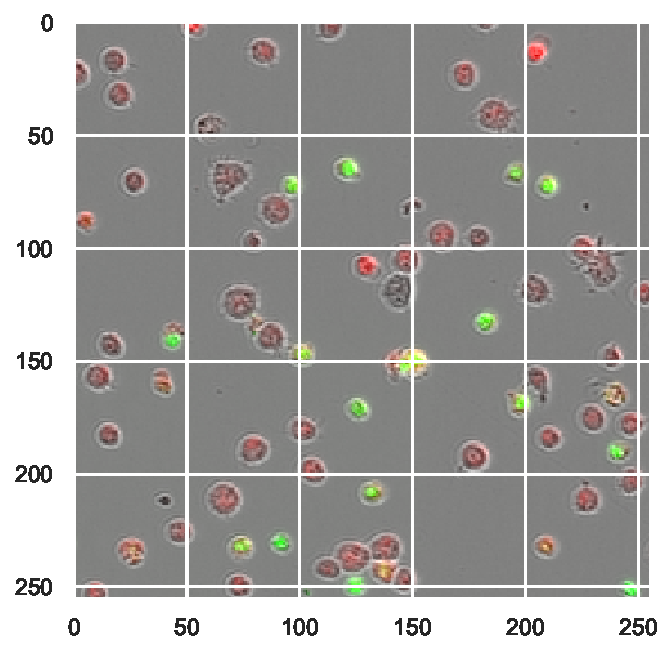
\includegraphics[width=.45\linewidth]{img/nms_full_colour.pdf}}}%
\caption{The processing of a test image: phase contrast input image (a); raw model bounding box predictions (b); non-maximum suppression post-processing (c); finally, for comparison, the corresponding full fluorescence image (d).}
\label{fig:nms}
\end{figure}

Following \cite{sermanet2013overfeat} we designed our network to be \emph{fully convolutional} (FCN). A FCN is capable of performing inference on any size of input, and is extended naturally to object detection. Thus, once trained on cell crops as a classifier, inference may be performed on an entire image in a single forward pass, producing a map of softmax probabilities at every location in the image. Note that even on CPU, a full $1408 \times 1040$px image is processed by the network in about $1$s.  Fully-convolutional whole-image inference emulates sliding-window detection, albeit without the tremendous inefficiency of executing the model separately at every spatial position. Note that the resolution of the output will depend on the number of pooling layers in the network. For example, our network includes two max pooling layers, hence we make detections at a stride of $4$ across the input image domain.

%We justify our choice of network by benchmarking against against cross-validated SVM (0.89 mean precision and 0.89 mean recall on balanced data) and random forest baseline models (0.89 mean precision and 0.88 mean recall). Note that neither of these can be used efficiently in a sliding window fashion as the CNN can. Moreover, the network outperforms the baselines (0.96 mean recall and 0.96 mean precision)



%\subsection{Calibrating posterior probabilities}
%
%Class imbalance is a challenge in our application as cells are seeded at different proportions depending on the experiment. Furthermore, cell behaviours such as mitosis often outpace cell death, leading to a trend towards imbalance over the course of the experiment. We require our system to be agnostic with respect to class priors, $\pi_0$ and $\pi_1$ (negative and positive classes).
%
%%\begin{figure}[htb]
%%\includegraphics[width=8.5cm]{img/confusions.pdf}
%%\caption{Confusion matrices for the same classifier on balanced data (left) and unbalanced data (right). The .}
%%\label{fig:confusions}
%%\end{figure}
%
%In Figure \ref{fig:confusions} we see how errors accumulate when a network trained on balanced data is confronted with an imbalanced dataset. Although the classifier has 95, $\pi_0 >> \pi_1$ leads to an abundance of false positives (116), a  . To mitigate this. effect \cite{dal2015calibrating} propose a calibration formula with posterior probabilities. Let denote $C_0$ and $C_1$ represent regions of feature space for class 0 and class 1 respectively where, $C_0 = \big\{\mathbf{x} : p(C = c_0 \ | \ \mathbf{x}) \geq \rho)\big\}$ and, $C_1 = \big\{\mathbf{x} : p(C_1 \ | \ \mathbf{x}) \leq \rho)\big\} = \big\{\mathbf{x} : p(C_0 \ | \ \mathbf{x}) \geq 1 - \rho)\big\}$ for some probability level $\rho$. Now define the set, $\mathcal{M} = C_0 \cap C_1 = \big\{\mathbf{x} \ : \ p(C_0 \ | \ \mathbf{x}) = \rho\big\}$. This defines a particular probability contour between the classes e.g. a decision boundary. Denote class priors $\pi_0 = p(C_0)$ and $\pi_1 = p(C_1)$. By Bayes' theorem,
%
%$$p = \frac{\pi_0p(\mathcal{M} \ | \ C_0)}{\pi_0p(\mathcal{M} \ | \ C_0) + \pi_1p(\mathcal{M} \ | \ C_1)}$$
%
%where $p = p(C_0 \ | \ \mathcal{M})$ is the posterior probability. If the priors change, the conditional probabilities do not change, but the posteriors do,
%
%$$p' = \frac{\pi_0'p(\mathcal{M} \ | \ C_0)}{\pi_0'p(\mathcal{M} \ | \ C_0) + \pi_1'p(\mathcal{M} \ | \ C_1)}$$
%
%where $p' = p(C_0 \ | \ \mathcal{M}, \pi_0'$, $\pi_1')$ given adjusted priors $\pi_0'$ and $\pi_1'$. Rearranging (1) above gives,
%
%$$p(\mathcal{M} \ | \ C_1) = \frac{\pi_0}{\pi_1}\bigg(\frac{1}{p} - 1\bigg) p(\mathcal{M} \ | \ C_0) $$
%
%Substituting into (2) gives,
%
%$$p' = \frac{\beta p}{\beta p + \beta' - \beta' p}$$
%
%where $\beta = \pi_1/\pi_0$ and $\beta' = \pi_1'/\pi'_0$ i.e. the ratio of positive cases in each rebalancing of the problem. Note that in the particular case of $\pi_0' = \pi'_1$ (balanced dataset), we get,
%
%$$p' = \frac{\beta p}{\beta p + 1 - p}$$
%
%This has the effect of shifting the decision boundary to regions where there is a more even chance of either class.

%\begin{figure}
%\centering
%\begin{tikzpicture}[font=\sffamily]
%\node (A) at (0, 0) {\tiny$(14, 14, 1)$};
%\node (B) at (2, 0) {\tiny$(12, 12, 16)$};
%\node (C) at (4, 0) {\tiny$(10, 10, 32)$};
%\node (D) at (6, 0) {\tiny$(5, 5, 32)$};
%\node (E) at (8, 0) {\tiny$(3, 3, 64)$};
%\node (F) at (10, 0) {\tiny$(1, 1, 64)$};
%\node (G) at (12, 0) {\tiny$(1, 1, K)$};
%\draw [->] (A) -- node [above=0.2cm, align=center] {\tiny{conv$_{3\times 3} \circ \sigma$}} (B);
%\draw [->] (B) -- node [above=0.2cm, align=center] {\tiny{conv$_{3\times 3} \circ \sigma$}} (C);
%\draw [->] (C) -- node [above=0.2cm, align=center] {\tiny{maxpool$_{2\times 2}$}} (D);
%\draw [->] (D) -- node [above=0.2cm, align=center] {\tiny{conv$_{3\times 3} \circ \sigma$}} (E);
%\draw [->] (E) -- node [above=0.2cm, align=center] {\tiny{conv$_{3\times 3} \circ \sigma$}} (F);
%\draw [->] (F) -- node [above=0.2cm, align=center] {\tiny{conv$_{1\times 1} \circ \sigma$}} (G);
%%\draw[-Latex] (A) to (B);
%%\draw[-Latex] (B) to (C);
%%\draw[-Latex] (C) to (D);
%%\draw[-Latex] (D) to (E);
%%\draw[-Latex] (E) to (F);
%%\draw[-Latex] (F) to (G);
%%\draw[-Latex] (C) to (P);
%%\draw[-Latex] (B) to [out=20,in=160] (P);
%\end{tikzpicture}
%\caption{Fully convolutional network architecture. We here illustrate the evolution of the tensor for an input shaped $(14, 14, 1)$, that is, a $14 \times 14$ crop with a single channel. $K$ is the number of classes modeled. The network is engineered to result in a scalar output. Increasing the input size will increase the output size. The function $\sigma$ is the non-linearity, chosen to be a rectified linear unit (ReLU).} 
%\end{figure}

At inference time, the object and conditional class probabilities are combined to give the marginal class probabilities $Pr(c) = Pr(c | o) \cdot Pr(o)$. Note that $Pr(c | \neg o) = 0$. These probabilities are thresholded and pruned with non-maximum suppression (NMS), providing a final detection mask for each class. For the NMS algorithm, we use an intersection over union threshold of 0.35. An example of this procedure is shown in Figure \ref{fig:nms}.

\subsubsection{Smoothing probabilities in time}

Because the cells are relatively stationary, we can improve the prediction of our system by leveraging information across time. We find a simple weighted average of prediction probabilities from consecutive frames, computed prior to NMS, improves overall performance. We thus define the \emph{smoothed} probability $p_{ij}^{(t)} \leftarrow 1/4\cdot p_{ij}^{(t-1)} + 1/2\cdot p_{ij}^{(t)} + 1/4 \cdot p_{ij}^{(t+1)}$ for the probability at image position $(i, j)$ at time $t$. The weights were tuned manually for both performance and parsimony.

%\begin{figure}[htb]
%\includegraphics[width=8.5cm]{img/umap.pdf}
%\caption{UMAP\cite{mcinnes2018umap} visualisations of living (red) and dead (green) Raji cells and background crops (blue) as model inputs (left) and hidden representations (right).}
%\label{fig:umap}
%\end{figure}

%\subsection{Training strategy \#2 - dense detection}
%\label{subsec:dense}

%An alternative strategy to preselecting crops is to train directly on the image itself. We hypothesise that training may attenuate some of the biases connected with crop extraction such as the upsampling, and crude background sampling. Though a good object detection system requires a good constituent classifier, good classification alone may not imply a good object detector in practice. We therefore take a training approach of \emph{dense detection}. To achieve this, we take the segmentation from the ground truth and use the central pixel of each connected component as a marker, which we dilate for robustness, yielding a binary mask of detection markers for each class.
%
%At training time, the regions of the full image are sampled uniformly randomly in mini-batches at a tunable cropping size. We achieved best results for regions of size $28$px $\times 28$px, though a potential source of future work is to explore the effect of varying this size. The output of the network is now a probability tensor, which a softmax preformed at every spatial location. To better account for the class imbalance, we replace the vanilla cross entropy used in the previous training procedure with a focal loss function \cite{lin2018focal}, specifically designed for dense detection. The focal loss for a data sample $\mathbf{x}$ is defined as,
%
%\[
%\mathcal{L}_{focal} = -\alpha_t(1 - p_t)^\gamma\log p_t
%\]
%
%where $p_t = f(\mathbf{x})_t$ is the probability emitted by the model $f$ corresponding to the ground truth label $t$ for example $\mathbf{x}$, $\alpha_t$ is a corresponding weight to address class-imbalance (that we set to the inverse class probability), and $\gamma$ is a tunable hyper-parameter (we set $\gamma = 2$). As such, the focal loss is a sort of modulated cross entropy, down-weighting probabilities close to 1 (those examples about which the model is sure) to dampen their superfluous influence on learning. It therefore embodies a learning strategy analogous to boosting methods, devoting greater attention to hard-to-classify examples. Once trained, the network is used as an object detector as in Section \ref{subsec:crops}.

\subsection{Results}
\label{subsec:results}

\subsubsection{Evaluation strategy}
\label{subsubsec:evaluation}

To evaluate our system, we manually annotated three days worth of frames of size $256 \times 256$px from each of two independent experimental replicates, totaling 72 images and approximately 7,000 test object detections. The replicates were chosen to represent different population dynamics: the first exhibits higher levels of cell mitosis; the second exhibits higher levels of cell apoptosis. We henceforth refer to these two datasets as Mitosis and Apoptosis respectively. The annotations consist of manually annotated bounding boxes around the cells. We make this dataset publicly available along with the images used to train the network\footnote{\texttt{https://zenodo.org/record/3515446}}. Note that despite this manually annotated evaluation dataset, our model is still trained on a ground truth that is automatically generated from the experiment.

%The annotations form a binary mask per object class that we compare with the masks generated by the object detection system.

We score our detections in terms of the distance of the bounding box centers to the ground truth bounding box centers. We define the following metrics:

\begin{itemize}
\item True positive (TP) - a cell is detected in the vicinity of a ground truth cell.
\item False positive (FP) - a cell is detected outside the vicinity of any ground truth cell.
\item False negative (FN) - no cell is detected within the vicinity of a ground truth cell.
\end{itemize}

Here we define vicinity to be $\leq 10$px, the maximum distance a predicted cell center may fall from a ground true center while still falling within the typical cell bounding box ($14 \times 14$px). These metrics are computed per cell class, from which we calculate precision, recall, and $F_1$ scores. Note the $F_1$ score prevails over the commonly used Matthews correlation coefficient as it does not require us to define true negatives (a meaningless quantity in our framework). These are displayed in Tables \ref{table:mitosis} and \ref{table:apoptosis} for the Mitosis and Apoptosis test sets. We see the effect of smoothing is globally positive, significantly improving the precision of the dead cell class, and giving the highest average $F_1$ scores of $83.86$ for Mitosis and $81.19$ for Apoptosis. Note that the results on the dead cell class are markedly worse. We postulate this is due to the class imbalance at test time, as well as the difficulty of discerning individual cells from cell clusters.

\begin{table}[ht!]
\begin{center}
\begin{tabular}{|l|c|c|c|c|}
\hline
Method & Class & Precision & Recall & $F_1$\\
\hline
\multirow{2}{4em}{Without smoothing} & Living & $0.8534$ & $0.8636$ & $0.8585$ \\ 
 & Dead & $0.7179$ & $0.8693$ & $0.7864$ \\
\hline
\multirow{2}{4em}{With smoothing} & Living & $0.8466$ & $0.8883$ & $\mathbf{0.8669}$ \\ 
 & Dead & $0.7702$ & $0.8549$ & $\mathbf{0.8103}$ \\
\hline
\end{tabular}
\end{center}
\caption{Detection performance on the Mitosis test set, stratified by object class. Best results in bold.}
\label{table:mitosis}
\end{table}

\begin{table}[ht!]
\begin{center}
\begin{tabular}{|l|c|c|c|c|}
\hline
Method & Class & Precision & Recall & $F_1$\\
\hline
\multirow{2}{4em}{Without smoothing} & Living & $0.9451$ & $0.7778$ & $0.8533$ \\ 
 & Dead & $0.6253$ & $0.8935$ & $0.7357$ \\
\hline
\multirow{2}{4em}{With smoothing} & Living & $0.9447$ & $0.7957$ & $\mathbf{0.8638}$  \\ 
 & Dead & $0.6628$ & $0.8904$ & $\mathbf{0.7600}$ \\
\hline
\end{tabular}
\end{center}
\caption{Detection performance on the Apoptosis test set, stratified by object class. Best results in bold.}
\label{table:apoptosis}
\end{table}
 
%We see that the dense detection strategy is overall superior crop extraction approach. We believe this might be due to the ill-calibrated posteriors arising from the biases inherent in the training strategy. The dense detection approach also implicitly allows to view each cell at different shifts, and then to better understand the difference between foreground and background. The cropping strategy has a consistently higher recall, and we suspect the balanced training makes it overly eager to classify objects (at the expense of precision). Nevertheless, there is clear room for improvement for our dense detector, in particular for dead cells. We suspect there is a lot to be gained by tuning the various hyperparameters in our system, something we intend to pursue immediately.

%\begin{table*}[ht!]
%\begin{center}
%\begin{tabular}{|l|c|c|c|c|c|} 
%\hline
%Method & Class & Precision & Recall & $F_1$ \\
%\hline
%\multirow{2}{4em}{Without smoothing} & 0.70 & $\mathbf{0.96}$  & 0.81 & 0.44 \\ 
% & 0.29 & $\mathbf{0.90}$ & 0.44 & 0.44 \\
%\hline
%\multirow{2}{4em}{With smoothing} & $\mathbf{0.91}$ & 0.93 & $\mathbf{0.92}$ & 0.44 \\ 
% & $\mathbf{0.47}$ & 0.74 & $\mathbf{0.58}$ & 0.44\\
%\hline
%\end{tabular}
%\end{center}
%\caption{Comparison of training approaches, stratified by object class. GIVE ABSOLUTE ERROR OF POPULATION CURVES}
%\label{table:results}
%\end{table*}

%
%\begin{figure}[htb]
%\includegraphics[width=8.5cm]{img/sample.pdf}
%\caption{Full fluorescent image crop with live Raji cells in red and dead cells in green (left) compared with a typical sample detection result on phase contrast only (right). A dead cell false positive can be seen in the first row, second column of the grid, and a live cell false negative in the fourth row, third column of the grid.}
%\label{fig:detections}
%\end{figure}

\subsubsection{Tracking population numbers over time}
\label{subsubsec:tracking}
Our detection system is ultimately used to enumerate cell phenotypes over the course of CAR-T experiments. In Figure \ref{fig:populations} we plot ground truth population numbers against the numbers inferred by our system. One can see the increasing number of living cells in Figure \ref{fig:populations}(a), corresponding to increasing amounts of cell division, whereas in Figure \ref{fig:populations}(b), one can see increasing amounts of apoptosis. In the former, our system achieves a mean relative error percentage of $5.95\%$ and $5.56\%$ (resp. living and dead cells) and $5.81\%$ and $5.37\%$ in the latter.

\begin{figure}%
    \centering
    \subfloat[]{{\includegraphics[width=0.9\textwidth]{img/mitosis.pdf}}}%
    \qquad
    \subfloat[]{{\includegraphics[width=0.9\textwidth]{img/apoptosis.pdf}}}%
    \caption{Population curves for manually-annotated Mitosis test set (a) and Apoptosis test set (b), compared with detection system outputs.}
    \label{fig:populations}
\end{figure}

\subsection{Perspectives}
\label{subsec:perspectives}

In this paper we have shown the viability of predicting phenotypes in the absence of  fluorescence, as well as how fluorescence may be used to generate a robust ground truth for machine learning. We have trained a neural object detection system and tested it on two manually annotated datasets. We have also given an example of how time information can be incorporated into the prediction task. We feel the system can be further improved with a more precise and expanded dataset, something we intend to address in future work.

\section{Discussion on competing strategies}
\label{sec:discussion_strategies}

\label{sec:object_detection_system}

In this chapter we have compared two strategies for quantifying cells from phase contrast images, by leveraging paired fluorescence images. In Section \label{sec:fluorescent_labeling} we showed how image-to-image translation models (including a generative adversarial variant) could be used as fluorescent labelers, and could successfully synthesise the fluorescent channels corresponding to a phase contrast microscopy input. In Section \label{sec:object_detection_system} we took a different route, and showed how we could use fluorescence as the quasi-annotation of a training set for cell detector and classifier. In Figure \ref{fig:cells_wells} we compare the time series derived from applying each method on all fields of the plate, for the first $72$ hours of each time lapse movie. The fields are pooled to obtain a total count for each of the four replicate wells at each time point. The time series for the detection system are obtained simply by counting bounding boxes as in Section \ref{subsubsec:tracking}. For the fluorescence labeler, we require a more ad hoc approach. We cropped the central $1024 \times 1024$px of each frame and passed it through our labeler networks to generate the fluorescent images. We then performed a background subtraction using a mean filter to normalise the intensity levels, before thresholding to obtain a binary mask. We then simply count the number of non-zero pixels to obtain an index acting as proxy to the total number of cells. Figure \ref{fig:cells_wells} shows a strong correlation between the outputs of the two systems. This is corroborated in Table \ref{table:correlations}.

\begin{sidewaysfigure}
\centering
\includegraphics[width=\textwidth]{img/wells.pdf}
\caption{Comparing cell quantification strategy by accumulation of cell types over time in four well replicates, aggregating over fields of view. The labeling series are normalised to have the same mean as the detection series. The lines are the means taken over the four replicates and the shaded regions represent their $95\%$ confidence intervals.}
\label{fig:cells_wells}
\end{sidewaysfigure}

\begin{table}[h]
\begin{center}
\begin{tabular}{|c|c|c|}
\hline
Well & Alive & Dead \\
\hline
A01 & 0.9751 & 0.8935\\
A02 & 0.9851 & 0.8657\\
A05 & 0.9888 & 0.8230\\
A06 & 0.9734 & 0.8840\\
\hline
\end{tabular}
\end{center}
\caption{Correlations between object detection and fluorescence labeling time series for alive and dead Raji cells in four experimental replicates.}
\label{table:correlations}
\end{table}
